
\documentclass[11pt]{report}

\usepackage{graphicx}
\usepackage{framed}
\usepackage{listings}
\usepackage{titlesec}
\usepackage{tikz}
\usepackage{amssymb}
\usepackage{amsmath}
\usepackage{amsthm}
\usepackage{MnSymbol}
\usepackage{stmaryrd}
\usepackage{multirow}
\usepackage{rotating}
\usepackage{caption}
\usepackage{subcaption}
\usepackage[margin=1.4in]{geometry}
\usepackage{algorithm,algorithmic}
\newcommand{\chapterbreak}{\clearpage}
\usepackage{tabularx}

\lstset{frame=tb,
  language=Java,
  aboveskip=5mm,
  belowskip=5mm,
  showstringspaces=false,
  columns=flexible,
  basicstyle={\small\ttfamily},
  numbers=none,
  breaklines=true,
  breakatwhitespace=true
  tabsize=3
}


\newtheorem{theorem}{Theorem}[section]
\newtheorem{lemma}[theorem]{Lemma}
\newtheorem{proposition}[theorem]{Proposition}
\newtheorem{corollary}[theorem]{Corollary}

%\newenvironment{proof}[1][Proof]{\begin{trivlist}
%\item[\hskip \labelsep {\bfseries #1}]}{\end{trivlist}}
\newenvironment{definition}[1][Definition]{\begin{trivlist}
\item[\hskip \labelsep {\bfseries #1}]}{\end{trivlist}}
\newenvironment{example}[1][Example]{\begin{trivlist}
\item[\hskip \labelsep {\bfseries #1}]}{\end{trivlist}}
\newenvironment{remark}[1][Remark]{\begin{trivlist}
\item[\hskip \labelsep {\bfseries #1}]}{\end{trivlist}}



\newcommand{\pre}{\mathop{\mathrm{pre}}}
\newcommand{\myparagraph}[1]{\paragraph{#1}\mbox{}\\}



\begin{document}

\tableofcontents
\clearpage
\begin{abstract}

\end{abstract}

\chapter{Introduction}

Verifying computer systems is essential. They have become such an important part of our lives that unforeseen software bugs and malfunction can lead to disastrous situations. One of many examples is the 1996 Arianne \textrm{V} satellite launcher, whose internal software caused the self-destruction of the module as a result of a simple but erroneous float-to-integer conversion. Another example of bad software is the Therac-25 radiation therapy machine, which massively overdosed six patients between 1985 and 1987, causing the death of at least three of them. 

Our dependency on computer systems is increasing, but so is their \textit{complexity} which, more often than not, demands a large amount of skilled human maintenance. Financially, this has motivated the need for systems to be more independent, and consequently, a large number of the critical systems that we rely on are now \textit{autonomous}: they are able to ``make decisions" without human intervention, based on a variety of factors such as their current state or environment. 

For the majority of current software systems, the verification is done by manual or automated \textit{testing}, with limited efficiency, as it is generally impossible to test \textit{all} possible situations. This is even more true in the case of autonomous systems, where the number of situations which might occur is much higher than usual. In the context of safety-critical systems, we want to be able to \textit{prove} that they meet their specification, and function correctly without bugs.

The verification of autonomous systems has been a very active research area in the past few decades due to their rising importance, and a range of verification techniques have been developed based on formal methods for modelling systems, including automated theorem proving or \textit{model checking}, the latter being the focus of this project.
\\\\
 Model checking was introduced in 1981 by E. M. Clarke and E. A. Emerson \cite{original_model_checking}, and independently by J. P. Queille and J. Sifakis \cite{symbolic_model_checking}, and is found to have major advantages \cite{birth_of_model_checking}: no correctness proofs are required (it is an automatic process), it finds counterexamples (i.e. bugs), and it allows for many different properties to be checked, by means of temporal logics. 
 
Unfortunately, an important disadvantage of model checking, known as the \textit{state explosion problem}, is the difficulty in verifying larger systems efficiently. In the past 20 years, several techniques attempting to solve the state explosion problem have been introduced, such as predicate abstraction, bounded model checking, symmetry reduction, and (perhaps more notably, at least for this project) symbolic model checking with \textit{ordered binary decision diagrams} (OBDDs, \cite{bryant}).

The idea of symbolic model checking, introduced in 1992 by K. L. McMillan \cite{symbolic}, is to encode states and transitions of the system as \textit{Boolean functions}, and represent these symbolically using efficient and compact data structures such as OBDDs. Symbolic model checking with OBDDs has allowed for very large systems to be verified, and has therefore seen a rise in the popularity of model checking as a verification technique.
Although OBDD-based techniques have significantly improved the efficiency of model checking, they have limitations and only allow systems up to about $10^{20}$ states to be verified \cite{1020_beyond}. Beyond, the OBDDs generated become too large to be efficiently handled by today's computers. 
\\\\
Several alternatives have been proposed to the use of OBDDs in symbolic model checking. In particular, a number of SAT-based methods have been introduced \cite{sat_based_smc3, sat_based_smc, sat_based_smc2}, demonstrating potential to outperform OBDDs in some situations, though these tend to focus on \textit{bounded} model checking, which only verifies part of a system. 

On the other hand, no other \textit{representations} of Boolean functions have been as influential as OBDDs in symbolic model checking. Experiments have been conducted with 

, and some recent results \cite{evmdd, multivalued_data_structures} have proposed the symbolic encoding of systems using multi-valued logics, leading to potentially more compact representations.
 
In this project, we explore the possibility of replacing OBDDs with a new symbolic representation of (classical two-valued) Boolean functions known as the \textit{sentential decision diagram} (SDD), first introduced in 2011 by A. Darwiche \cite{sdd_1}. SDDs were originally introduced as an alternative data structure in the field of \textit{knowledge compilation} and, until this project, they had never been experimented with in the context of model checking. 

\section{Contributions}

This project constitutes a first investigation of the use of sentential decision diagrams in symbolic model checking. Our contributions include: 
\begin{enumerate}
\item A theoretical approach to model checking with SDDs, determining the different aspects of the process and the choices involved;
\item An implementation of a model checker for multi-agent systems entirely based on SDDs;
\item Some heuristics for a more efficient use of SDDs in model checking multi-agent systems;
\item A thorough comparison of the above with OBDD-based model checking.
\end{enumerate}




\chapter{Background}

\section{Logics for Multi-Agent Systems}

\subsection{Multi-Agent Systems}

Autonomous multi-agent systems are computer systems which are made up of several intelligent ``agents" acting within an ``environment". 
Intuitively, an \textit{agent} is: 
\begin{itemize}
\item Capable of \textit{autonomous} action 
\item Capable of \textit{social} interaction with its peers
\item Acting to \textit{meet} their design objectives 
\end{itemize}
 
Suppose we have a multi-agent systems consisting of $n$ agents and an environment $e$.
\begin{definition} 
An agent $i$ in the system consists of: 
\begin{itemize}
\item A set $L_i$ of local states representing the different configurations of the agent,
\item A set $Act_i$ of local actions that the agent can take,
\item A protocol function $P_i : L_i \rightarrow 2^{Act_i} $ expressing the decision making of the agent.
\end{itemize} 
\end{definition}

We can define the environment $e$ as a similar structure $(L_e, Act_e, P_e)$ where $P_e$ represents the functioning conditions of the environment. 

\subsection{Interpreted Systems}
\label{IS}
We present a formal structure to represent multi-agent systems. Consider a multi-agent system $\Sigma$ consisting of $n$ agents $1, ..., n$ and an environment $e$.
\begin{definition}
An \textit{Interpreted System} $IS$ for $\Sigma$ is a tuple $(G, \tau, I, \sim_1, ..., \sim_n, \pi)$, where
\begin{itemize}
\item $G \subseteq L_1 \times ... \times L_n \times L_e$ is the set of global states that $\Sigma$ can reach. A global state $g \in G$ is essentially a picture of the system at a given point in time, and the local state of agent $i$ in $g$ is denoted $l_i(g)$.
\item $I \subseteq G$ is a set of intial states for the system
\item $\tau : G \times Act \rightarrow G $ where $Act = Act_1 \times ... \times Act_n \times Act_e$ is a deterministic transition function (we can define $\tau : G \times Act \rightarrow 2^G$ to model a non-deterministic system)
\item $\sim_1, ..., \sim_n \subseteq G \times G$  are binary relations defined by $$g \sim_i g' \Leftrightarrow l_i(g) = l_i(g') \quad \forall g, g' \in G, \forall i = 1, ..., n$$
i.e iff agent $i$ is in the same state in both $g$ and $g'$. 
\item $\pi : PV \rightarrow G$ is a valuation function for the set of atoms $PV$, i.e for each atom $p \in PV$, $\pi(p)$ is the set of global states where $p$ is true
\end{itemize}
\end{definition}
We also need a formal definition for the ``execution'' of a system. A \emph{run}, as defined below, represents one possible execution of a MAS. 
\begin{definition} 
A \emph{run} of an interpreted system $IS = (G, \tau, I, \sim_1, ..., \sim_n, \pi)$ is a sequence $r = g_0, g_1, ...$ where $g_0 \in I$ and such that for all $i \geq 0$, $\exists a \in Act$ such that $\tau(g_i, a) = g_{i+1}$.
\end{definition}

Interpreted systems as defined above are used as semantic structures for a particular family of logics, presented in the next section.

\subsection{Linear Temporal Logic} 
\label{LTL}

In order to verify properties of multi-agent systems, we first need to find a logic allowing us to describe these properties accurately. 

A good candidate is the Linear Temporal Logic (LTL), a modal temporal logic in which one can write formulas about the future of \emph{paths}. Here we use paths to represent infinite runs of an interpreted system. 

\begin{definition} 
The syntax of LTL formulas is given by the following BNF: 
$$\varphi := p \mid \lnot\varphi \mid \varphi \land \varphi \mid X\varphi \mid G\varphi \mid \varphi U\varphi$$
\end{definition}

The intuitive meanings of $X\varphi, G\varphi$ and $\varphi U\psi$ are respectively 
\begin{itemize} 
\item $\varphi$ holds at the ne\textbf{X}t time instant
\item $\varphi$ holds forever (\textbf{G}lobally)
\item $\varphi$ holds \textbf{U}ntil $\psi$ holds  
\end{itemize}

We define the unary operator $F$ to be the dual of $G$, i.e $F\varphi := \lnot G\lnot\varphi$ for any LTL formula $\varphi$. $F\varphi$ represents the idea that $\varphi$ will hold at some point in the \textbf{F}uture.   

\myparagraph{Semantics} 

A model for LTL is a Kripke model $M = (W, R, \pi)$ such that the relation $R$ is serial, i.e $\forall u \in W,  \exists v \in W$ such that $(u, v) \in R$.
The worlds in $W$ are called the \textit{states} of the model. 

\begin{definition} 
A \textit{path} in an LTL model $M = (W, R, \pi)$ is an infinite sequence of states $\rho = s_0, s_1, ...$ such that $(s_i, s_{i+1}) \in R$ for any $i \geq 0$.
We denote $\rho^i$ the suffix of $\rho$ starting at $i$ (note that $\rho^i$ is itself a path since $\rho$ is infinite).
\end{definition}

It is easy to see how such a model can be used to represent a computer system, and how an execution of this system can be written as a path.

 Our objective is to be able to verify that a system $S$ has property $P$, so if we encode $P$ as an LTL formula $\varphi_P$ and $S$ as a model $M_S$, then we need to be able to check whether $\varphi_P$ is \textit{valid} in $M$ (or at least true in a set of initial states). This technique is called \textit{model checking}, and we do this by using the following definition for the semantics of LTL:
\label{model_checking}

\begin{definition}
Given LTL formulae $\varphi$ and $\psi$, a model $M$ and a state $s_0 \in W$, we say that
\begin{eqnarray*}
(M, s_0) \models p &\Leftrightarrow& s_0 \in \pi(p) \\  
(M, s_0) \models \lnot \varphi &\Leftrightarrow& (M, s_0) \nmodels \lnot \varphi\\
(M, s_0) \models \varphi \land \psi &\Leftrightarrow& (M, s_0) \models \varphi \mbox{ and  } (M, s_0) \models \psi \\
(M, s_0) \models X\varphi &\Leftrightarrow& (M, s_1) \models \varphi \mbox{  for all states } s_1 \mbox{ such that } R(s_0, s_1)\\
(M, s_0) \models G\varphi &\Leftrightarrow& \mbox{for all paths } \rho = s_0, s_1, s_2, ... , \mbox{ we have } (M, s_i) \models \varphi \quad \forall i \geq 0 \\
(M, s_0) \models \varphi U\psi &\Leftrightarrow& \mbox{for all paths } \rho = s_0, s_1, s_2, ..., \exists j \geq 0 \mbox{ such that }  (M, s_j) \models \psi \\ && \mbox{ and }  (M, s_k) \models \varphi \quad \forall 0 \leq k < j
\end{eqnarray*}

\end{definition}
The expressive power of LTL is limited to quantification over \textit{all} possible paths. For example: 

\begin{itemize}
\item $FG($deadlocked$)$ 

In every possible execution, the system will be permanently deadlocked.


\item $GF($crash$)$

Whatever happens, the system will crash infinitely often.
\end{itemize}
Hence some properties cannot be expressed in LTL, as in certain applications we might want to quantify explicitely over paths. The Computation Tree Logic (CTL) can express this. 

\subsection{Computation Tree Logic} 

\begin{definition} 
The syntax of CTL formulae is defined as follows: 
$$ \varphi := p \mid \lnot \varphi \mid \varphi \land \varphi \mid EX\varphi \mid EG\varphi \mid E(\varphi U \varphi)$$
\end{definition}

Intuitively, $ EX\varphi,  EG\varphi,$ and $ E(\varphi U \psi)$ represent the fact that there exists a possible path starting from the current state such that, respectively, $\varphi$ is true at the next state, $\varphi$ holds forever in the future, and $\varphi$ holds until $\psi$ becomes true.

The dual operator $AX\varphi := \lnot EX \lnot\varphi $ can be used to represent the fact that in all possible paths from the current state, $\varphi$ is true at the next state.
Connectives $AG\varphi, AF\varphi,$ and $A(\varphi U\psi)$ can be defined in the same way. 

We also use models (as defined in \ref{LTL}) for the semantics of CTL, as follows:

\begin{definition} 
Given CTL formulas $\varphi$ and $\psi$, a model $M = (W, R, \pi)$ and a state $s_0 \in W$, the satisfaction of formulas at $s_0$ in $M$ is defined inductively as follows: 
\begin{eqnarray*}
(M, s_0) \models p &\Leftrightarrow& s_0 \in \pi(p) \\  
(M, s_0) \models \lnot \varphi &\Leftrightarrow& (M, s_0) \nmodels \lnot \varphi\\
(M, s_0) \models \varphi \land \psi &\Leftrightarrow& (M, s_0) \models \varphi \mbox{ and  } (M, s_0) \models \psi \\
(M, s_0) \models EX\varphi &\Leftrightarrow& \exists \mbox{ a path } s_0, s_1, s_2, ... \mbox{ such that } (M, s_1) \models \varphi \\
(M, s_0) \models EG\varphi &\Leftrightarrow& \exists \mbox{ a path } s_0, s_1, s_2, ... \mbox{ such that } (M, s_i) \models \varphi \quad \forall i \geq 0\\
(M, s_0) \models E(\varphi U\psi) &\Leftrightarrow&  \exists \mbox{ a path } s_0, s_1, s_2, ... \mbox{ for which } \exists i \geq 0 \mbox{ such that }  (M, s_i) \models \psi \\ && \mbox{ and }  (M, s_j) \models \varphi \quad \forall 0 \leq j < i
\end{eqnarray*}
\end{definition}
The quantifiers allow for more properties to be expressed, for example:
\begin{itemize}

\item $EF(AG($deadlocked$))$

It is possibly to reach a point where the process will be permanently deadlocked.

\item $AG(EX($reboot$))$ 

From any state it is possible to reboot the system.


\end{itemize}
Again, some formulas can be expressed in LTL but not in CTL. For instance, the property that \textit{in every path where $p$ is true at some point then $q$ is also true at some point} is expressed in LTL as $Fp \rightarrow Fq $ but there is no equivalent CTL formula.
 The logic CTL* combines the syntax of LTL and CTL to provide a richer set of connectives. We will not go into any more details regarding CTL*, but we refer the reader to \cite{ctl*} for more information. 

\subsection{The Epistemic Logic CTLK}

In the case of multi-agent systems, we are interested in describing the system in terms of individual agents, and in particular their \textit{knowledge}. 

For this reason, we can add \cite{ctlk} a family of unary operators $K_i$ for $i = 1, ..., n$ to the modal connectives defined previously. Each $K_i$ will represent the intuitive notion of knowledge for agent $i$. 
This enables us to define the temporal-epistemic logics LTLK and CTLK, which are extensions of LTL and CTL, respectively. Here we leave out details about LTLK, as the practical applications we present later on only support CTLK. 



\begin{definition} 
The syntax of CTLK is defined by the following BNF: 
$$ \varphi := p \mid \lnot \varphi \mid \varphi \land \varphi \mid EX\varphi \mid EG\varphi \mid E(\varphi U \varphi) \mid  K_i\varphi \quad (i \in \{1, ..., n\})$$
\end{definition}  

We use interpreted systems (\ref{IS}) as semantic structures for CTLK. The satisfaction of a CTL formula on an interpreted system $IS$ is defined analogously to its satisfaction on a model $M$ whose worlds $W$ are the global states of $IS$, and whose relation function $R$ is the global transition function of $IS$. 
For example, $(IS, g_0) \models EX\varphi \mbox{  iff there is a run } r = g_0, g_1, g_2, ... \mbox{ of $IS$ such that } (IS, g_1) \models \varphi$.

The following definition completes the semantics of CTLK formulae:

\begin{definition}
Given an interpreted system $IS$, a global state $g$, an agent $i$ of $IS$, and a CTLK formula $\varphi$, we define
$$(IS, g) \models K_i \varphi \mbox{  iff  } \forall g' \in G, g \sim_i g' \Rightarrow (IS, g') \models \varphi$$

The connective $K_i$ expresses that agent $i$ \emph{knows} of the property $\varphi$ when the system's global state is $g$.

We extend the syntax and semantics of CTLK by adding two extra unary operators: $E$ (Everybody knows) and $C$ (Common knowledge), whose semantics are defined as follows:

\begin{eqnarray*}
(IS, g_0) \models E\varphi &\Leftrightarrow& (IS, g_0) \models K_i \varphi \quad \forall i = 1, ..., n \\
(IS, g_0) \models C\varphi &\Leftrightarrow&  (IS, g_0) \models \bigwedge^\infty_{k = 1} E^{(k)}\varphi \quad \\&& \mbox{ where } E^{(1)} = E \mbox{ and } E^{(j+1)} = EE^{(j)} \quad \forall j \geq 1
\end{eqnarray*}
\end{definition}


\section{Model Checking}

Model checking was briefly introduced in \ref{model_checking} as a automated verification technique, which can be used to check that a system $S$ satisfies a specification $P$. The technique involves representing $S$ as a logic system $L_S$ which captures all possible computations of $S$, and encoding the property $P$ as a temporal formula $\varphi_P$. 

The problem of verifying $P$ is then reduced to the problem of checking whether $L_S \vdash \varphi_P $. But we can now build a Kripke model $M_S = (W_S, R_S, \pi)$ such that $L_S$ is sound and complete over (the class of) $M_S$, so that $$L_S \vdash \varphi_P \Leftrightarrow M_S \models \varphi_P .$$ 
$M_S$ is the Kripke model representing all possible computations of $S$, i.e. $W_S$ contains all the possible computational states of the system and the relation $R_S$ represents all temporal transitions in the system. 

In the case of a multi-agent system as defined above, encoding $S$ as an interpreted systems of agents will satisfy the equivalence, and we can use CTLK to encode properties of the system to be checked. 

\subsection{Explicit Model Checking}

\label{explicit}
In this section we present a first approach to model checking, the so-called \textit{explicit} approach. Although the explicit model checking algorithm for CTL was in the original article on model checking by Clarke et al.\cite{original_model_checking}, its extension to multi-agent systems and CTLK is due to the work of Lomuscio et al. in \cite{mas_verification}.

Suppose that we want to check that a multi-agent system $\Sigma$ satisfies a propery $P$. If $IS$ is an interpreted system representing $\Sigma$, and $\varphi$ the CTLK formula corresponding to $P$, we need to verify that $(IS, s_0) \models \varphi$, for all initial states $s_0 \in I$.

Algorithmically it is more efficient \cite{need ref} to compute the set of global states $\llbracket\varphi\rrbracket$ of $IS$ where $\varphi$ is true, and check that $I \subseteq \llbracket\varphi\rrbracket$. 
Algorithm~\ref{algo} returns $\llbracket\varphi\rrbracket$ for any CTLK formula $\varphi$.

\begin{figure}

\begin{lstlisting}[mathescape]

function SAT($\varphi$) 
// returns $\llbracket\varphi\rrbracket$
if $\varphi = \top$: return $G$
if $\varphi = \bot$: return $\varnothing$
if $\varphi = p$: return $\pi(p)$ 
if $\varphi = \lnot\varphi_1$: return $G \setminus$SAT($\varphi_1$)
if $\varphi = \varphi_1\land\varphi_2$: return SAT($\varphi_1$)$\cap$SAT($\varphi_2$)
if $\varphi = EX\varphi_1$: return SAT$_{\mbox{EX}}(\varphi_1)$
if $\varphi = AF\varphi_1$: return SAT$_{\mbox{AF}}(\varphi_1)$
if $\varphi = E(\varphi_1 U\varphi_2 )$: return SAT$_{\mbox{EU}}(\varphi_1, \varphi_2)$
if $\varphi = K_i\varphi_1$: return SAT$_{\mbox{K}}(i, \varphi_1)$
if $\varphi = E\varphi_1$: return SAT$_{\mbox{E}}(\varphi_1)$
if $\varphi = C\varphi_1$: return SAT$_{\mbox{C}}(\varphi_1)$
end
$\\$
\end{lstlisting}
\caption{test}
\label{algo}
\end{figure}
Notice that this covers all formulae $\varphi$, as $\{EX, AF, EU, K_i, E, C\}$ is a minimum set of connectives for CTLK. The respective auxilliary functions are defined below. Notation: for any global states $g_0, g_1$ of $IS$ we write $g_0 \rightarrow g_1$ iff $\exists a \in Act$ such that $\tau(g_0, a) = g_1$ (i.e. there is an run of $IS$ starting with $g_0, g_1, ...$).

\begin{figure}
\begin{lstlisting}[mathescape]

function SAT$_{\mbox{EX}}$($\varphi$)
// returns $\llbracket EX\varphi\rrbracket$
  X := {$g_0 \in G \mid g_0 \rightarrow g_1$ for some $g_1 \in $SAT($\varphi$) }
  return X
end
 
function SAT$_{\mbox{AF}}$($\varphi$)
// returns $\llbracket AF\varphi\rrbracket$
  X := $G$
  Y := SAT($\varphi$)
  repeat until X = Y:
    X := Y
    Y := Y $\cup$ $\{ g_0 \in G \mid $ for all $g_1 $ with $g_0 \rightarrow g_1$, $g_1 \in$ Y $\}$ 
  end
  return Y
end
  

function SAT$_{\mbox{EU}}$($\varphi_1$, $\varphi_2$)
// returns $\llbracket E(\varphi_1U\varphi_2)\rrbracket$
  W := SAT($\varphi$)
  X := $G$
  Y := SAT($\psi$)
  repeat until X = Y:
    X := Y
    Y := Y $\cup$ (W $\cap$ $\{g_0 \in G \mid \exists g_1 \in$ Y such that $g_0 \rightarrow g_1\}$)
  end
  return Y
end
\end{lstlisting}
\end{figure}
\begin{figure}


\begin{lstlisting}[mathescape]

function SAT$_{\mbox{K}}$($i$, $\varphi$)
// returns $\llbracket K_i\varphi\rrbracket$
  X := SAT($\lnot\varphi$)
  Y := $\{g_0 \in G \mid \exists g_1 \in$ X with $g_0 \sim_i g_1\}$
  return $G \setminus\mbox{Y}$
end

function SAT$_{\mbox{E}}$($\varphi$)
// returns $\llbracket E\varphi\rrbracket$
  X := SAT($\lnot\varphi$)
  Y := $\{g_0 \in G \mid \exists g_1 \in$ X with $g_0 \sim_i g_1$ for all $i = 1, ..., n\}$
  return $G \setminus\mbox{Y}$
end

function SAT$_{\mbox{C}}$($\varphi$)
// returns $\llbracket C\varphi\rrbracket$
  X := $G$
  Y := SAT($\lnot\varphi$)
  repeat until X = Y:
    X := Y
    Y := $\{g_0 \in G \mid \exists g_1 \in$ X with $g_0 \sim_i g_1$ for all $i = 1, ..., n\}$
  end
  return $G \setminus\mbox{Y}$
end
$\\$
\end{lstlisting}
\end{figure}
The complexity of \texttt{SAT} is linear in the size of the model. However, the size of the model (i.e. the number of reachable states) grows exponentially in the number of variables used to describe the system $\Sigma$, therefore the explicit approach is not always viable in practice. This is the main difficulty in model checking and it is known as the \textit{state explosion problem}. 

Recall that in order to use the algorithm above we also need a way of computing the set of reachable states, which is rarely given explicitely. In most cases all that is given is the set $I$ of initial states of the system. The reachable state space can then be obtained by computing the fixed point of the transition relation function, as shown in the algorithm below:
\begin{figure}

\begin{lstlisting}[mathescape]

function compute_reach()
// returns the reachable state space $G$ 
  X := $\emptyset$
  Y := $I$
  repeat until X = Y
    X := Y
    Y := Y $\cup$  $\{ g_1 \in G \mid g_0 \rightarrow g_1 \mbox{ for some }g_0 \in X\}$
  end
  return Y
end
$$
\end{lstlisting}
\end{figure}

In the next section we introduce a model checking technique aiming to improve the efficiency of the approach. 



\subsection{Symbolic Model Checking}

\textit{Symbolic model checking} is an approach to model checking which involves representing sets of states and functions between them as Boolean formulas. The algorithm presented in \ref{explicit} is then reduced to a series of operations on Boolean formulas. In this section we go through the process of encoding sets and functions as propositional formulas, and we explain how this encoding facilitates model checking.

\myparagraph{Symbolic Representation of Sets of States}
\label{symbolic}
\begin{figure}
    \centering
    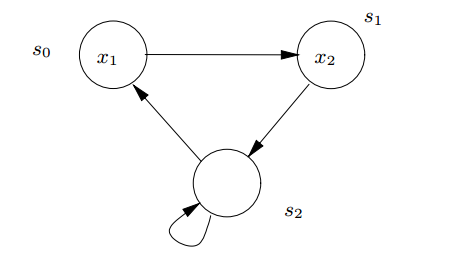
\includegraphics[scale=0.55]{symbolic_model_checking_example.PNG}
    \caption{A model}
    \label{fig:model_example}
\end{figure}

We use an example \cite{logic_in_computer_science} to illustrate the encoding process.
Consider the model in Figure~\ref {fig:model_example}, representing a system with three states labelled $s_0, s_1, s_2$. 

We consider two propositional variables, namely $x_1$ and $x_2$.  
If $S$ is the whole state space (so $S = \{s_0, s_1, s_2\}$), we can represent subsets of $S$ using Boolean formulae, as shown in the following table:\\

\vspace{0.3cm}
{\centering \begin{tabular}{ l | r }
  set of states & representation by boolean formula \\ \hline
$\emptyset $&   $\bot$ \\
$\{ s_0\}$ & $x_1 \land \lnot x_2 $\\
$\{ s_1\}$ & $ \lnot x_1 \land x_2 $\\
$\{ s_2\}$ & $\lnot x_1 \land \lnot x_2 $\\
$\{ s_0, s_ 1\}$ & $(x_1 \land \lnot x_2) \lor (\lnot x_1 \land x_2)  $\\
$\{ s_1, s_2\}$ & $(\lnot x_1 \land  x_2) \lor (\lnot x_1 \land\lnot x_2)$\\
$\{ s_0, s_2\}$ & $(x_1 \land \lnot x_2) \lor (\lnot x_1 \land\lnot x_2) $\\
$\{ s_0, s_1, s_2\}$ & $(x_1 \land \lnot x_2) \lor (\lnot x_1 \land  x_2) \lor (\lnot x_1 \land\lnot x_2)$
\end{tabular}
\\}
\vspace{0.3cm}



Note that for this representation to be unambiguous, we must ensure that no two states satisfy the same set of Boolean variables. If this is the case, new variables can be added which will be used to differenciate between the ambiguous states.


\subsubsection{Symbolic Representation of a Transition Relation}

The transition relation $\rightarrow$ of a model is a subset of $S \times S$. Taking two copies of our set of propositional variables, we can then associate a Boolean formula to the transition relation, as follows. 

Firstly, notice that in the example above the transition relation $\rightarrow$ of the model is $$\{(s_0, s_1), (s_1, s_2), (s_2, s_0), (s_2, s_2)\}.$$
Our set of Boolean variables was $\{x_1, x_2\}$; we now create a copy and use \textit{primed} variables to represent its elements. We get another set $\{x_1', x_2'\}$, which will be used to represent the \textit{next} state in our encoding of the transition relation.
Now, for each pair element in the set, we take the conjunction of the Boolean representation of each state in the pair, the first one using the original set of variables, the second the primed set. For example, with $(s_0, s_1)$ is associated the formula $(\lnot x_1 \land \lnot x_2) \land (\lnot x'_1 \land \lnot x'_2)$ (using the Boolean representation for $s_0, s_1$ derived above -- see the table).

As in the representation of sets of states, we represent sets of pairs by taking the conjunction of the representation of each pair element. Thus we compute the representation of $\rightarrow$ to be $(\lnot x_1 \land \lnot x_2 \land \lnot x'_1 \land \lnot x'_2 ) \lor (\lnot x_1 \land \lnot x_2 \land x'_1 \land \lnot x'_2 ) \lor ( x_1 \land \lnot x_2 \land \lnot x'_1 \land  x'_2 ) \lor (\lnot x_1 \land x_2 \land \lnot x'_1 \land \lnot x'_2 )$.

\subsubsection{Set Operations with Boolean Functions}

If sets of states are represented by Boolean functions, we need a way of applying equivalent operations to the Boolean functions in order to represent their union, intersection, or complement. It turns out that the definition of the symbolic representation of sets of states gives a natural correspondence between the basic set operations and the basic Boolean operations, as follows. 
Suppose that $X, Y$ are sets represented by Boolean functions $f_X$ and $f_Y$. Then
\begin{align*}
f_{X \cup Y} &= f_X \lor f_Y\\
f_{X \cap Y} &= f_X \land f_Y \\
f_{G\setminus X} &= \lnot f_X.
\end{align*}

\subsubsection{The Functions $\pre_\exists$ and $\pre_\forall$}

We have seen that the explicit model checking algorithm relies on two functions on sets of states, $$\mbox{pre}_{\exists} (X) = \{g_1 \in G \mid \exists g_0 \in X \mbox{ with } g_0 \rightarrow g_1\}$$ and $$\mbox{pre}_\forall (X) = \{g_1 \in G \mid\mbox{ if }g_0 \rightarrow g_1,\mbox{ then }g_0 \in X\}.$$ We therefore need a way of implementing those using the symbolic representations of sets of states introduced above. First note that $$\mbox{pre}_\forall (X) = G \setminus \mbox{pre}_{\exists} (G \setminus X),$$ so it is enough to have an algorithm for computing $\mbox{pre}_{\exists}(X)$ on a given set~$X$. Let us first recall a basic definition about Boolean functions:

\begin{definition}
\label{exist}
Let $f$ be a Boolean function. The \textit{conditioning} of $f$ on a variable $x$, written $f|_x$, is the Boolean function obtained by changing $x$ to $\top$ in $f$, and similarly $f|_{\lnot x}$
is obtained from $f$ by setting $x$ to $\bot$.
The \textit{existential quantification} of $f$ with respect to $x$, denoted $\exists x f$, is used to relax the constraint on variable $x$ in $f$, and it is defined by $$\exists x f = f|_x \lor f|_{\lnot x}.$$
\end{definition}

Suppose now that $X \subseteq G$ is a set of states encoded by function $f_X$, and that the transition relation $\rightarrow$ of the system is encoded by function $f_\rightarrow$. The algorithm has the following steps:
\begin{enumerate}
\item Rename variables in $f_X$ to their primed counterparts, and call the resulting function $f_{X'}$. 
\item Compute $f_{\rightarrow X'} = f_{X'} \land f_\rightarrow$.
\item Existentially quantify all primed variables away from $f_{\rightarrow X'}$, i.e. compute $\exists x_1' ... \exists x_n' f_{\rightarrow X'}.$ The resulting function is $f_{\mbox{pre}_\exists(X)}$, the symbolic representation of $\mbox{pre}_\exists(X)$.
\end{enumerate}
In the \texttt{compute\_reach} algorithm above, we use a different operator, which computes the set of states \textit{following} $X$ in the transition relation. This can be encoded in terms of Boolean functions in a very similar way: start with the Boolean encoding of $X$, conjoin with the encoding of the transition relation, existentially quantify all non-primed variables, and ``un-prime" the variables in the resulting function.

\subsubsection{The Case of Multi-Agent Systems}

Notice that the procedure described above is only valid for global states and does not distinguish between different agents. 
In the case of multi-agent systems, we can encode the local states for agents using the same method as for states in the general case, making sure to use a different set of variable for each agent. A Boolean representation for a global state in the system will then be the conjunction of the formulas for the local states of which it consists. The separate encoding of the states for each agent will also enable the agent protocols to be encoded independently.

Moreover, in order to successfully implement our model checking algorithm using symbolic expressions, we need a way of representing the agent accessibility relations $\sim_i$.
But each of these is a binary relation on states, i.e. a subset of $S \times S$. Hence we can use the exact same method as for the global transition relation. 
\\\\

How does this help us? Well, several techniques exist which allow us to represent these Boolean formulas in a very concise form. This is the topic of the next section.

\section{Representing Boolean functions}

It is important to make the point that the Boolean formulas computed in \ref{symbolic} can be regarded as Boolean \textit{functions}, i.e. functions $\{0, 1\}^n \rightarrow \{0, 1\}$ for some $n$. For example, the formula $x_1 \land \lnot x_2$ is associated to the function $f(x_1, x_2) = x_1 \land \lnot x_2$.

In this section we introduce various representations of Boolean functions using directed acyclic graphs (DAG). 

\subsection{Ordered Binary Decision Diagrams}

One the most basic ways of representing a Boolean function is by using a \textit{binary decision tree} (BDT). A BDT is a binary tree where we label non-terminal nodes with Boolean variables $x_1, x_2, ...$ and terminal nodes with the values 0 and 1. Each non-terminal node has two outgoing edges, one solid and one dashed (one for each value of the variable the node is labelled with). An example is shown in Figure~\ref{fig:BDT}. Note that the initial ordering of the variables affects the resulting BDT; for convenience, we write $[x_1, x_2, ..., x_n]$ to denote the order $x_1 < x_2 < ... < x_n$.

\begin{figure}
\centering
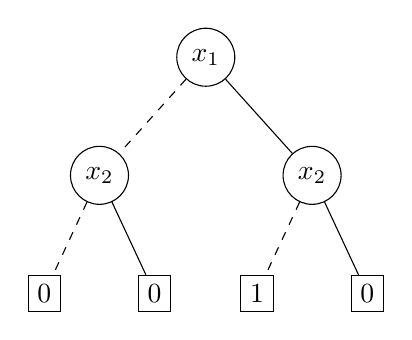
\begin{tikzpicture}

	\node[circle, draw] (x1) {$x_1$}	 [sibling distance=27mm]
		child {node[circle,draw] (x21) {$x_2$} [sibling distance=14mm][dashed]
			child {node[rectangle, solid, draw] (1) {0} [dashed]}
			child {node[rectangle, solid, draw] (01) {0} [solid]}}
		child {node[circle,draw] (x22) {$x_2$} [sibling distance=14mm][solid]
			child {node[rectangle, solid, draw] (02) {1} [dashed]}
			child {node[rectangle, solid, draw] (03) {0} [solid]}};
\end{tikzpicture}
	\caption{BDT for $f(x_1, x_2) = x_1 \land \lnot x_2$ under the ordering $[x_1, x_2]$}
\label{fig:BDT}
\end{figure}

BDTs are a relatively inefficient way of storing Boolean formulas, since a BDT for a formula with $n$ variables has $2^{n+1} - 1$ nodes. 
A binary decision diagram (BDD) is a directed acyclic graph, similar to a BDT but allowing nodes to have more than one incoming edge. A BDD is called an \textit{ordered binary decision diagram} (OBDD) if every path from the root to a terminal node, variables appear in the same order (although not all variables have to occur in the path). An extremely useful property of  OBDDs is that they can be \textit{reduced} to a ROBDD which is, in most cases, a far smaller data structure than the BDT for the same function. 
\begin{figure}
\centering
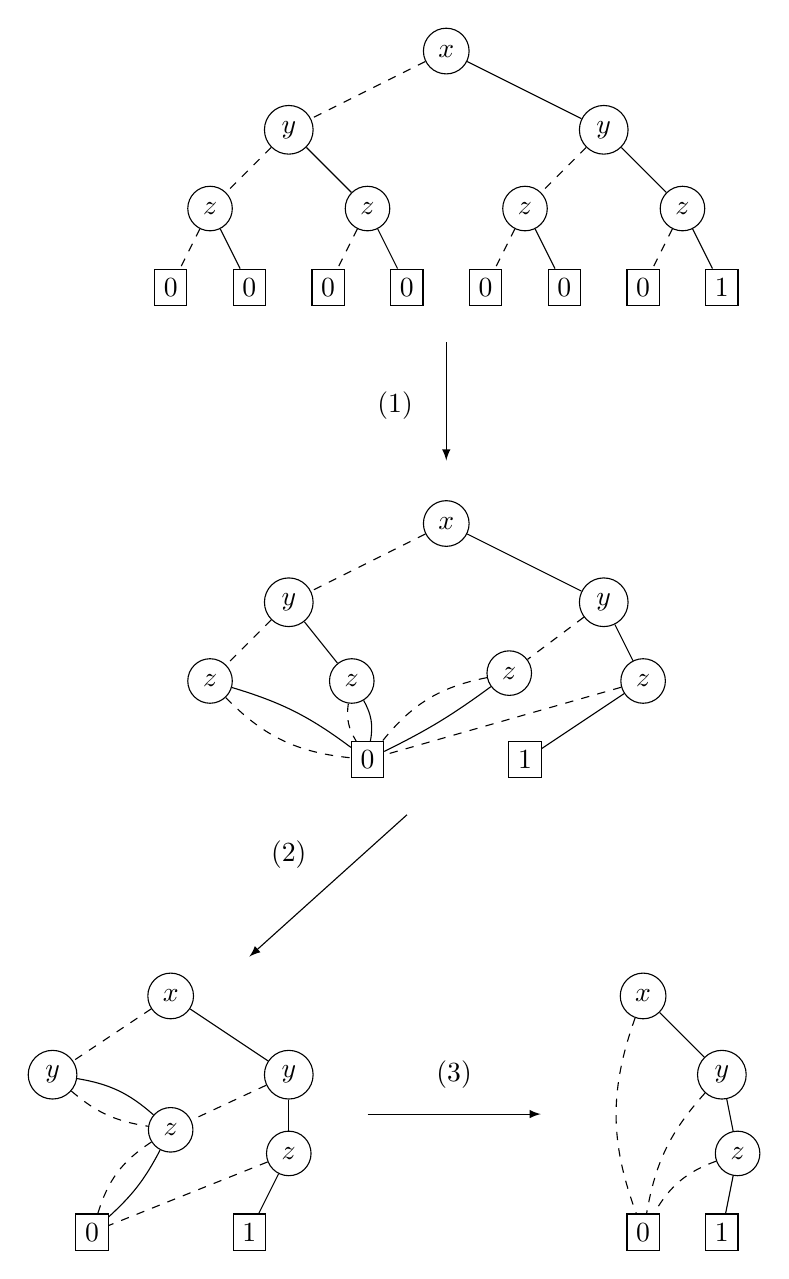
\begin{tikzpicture}
\node[draw, rectangle] (01) at (0,0) {0};
\node[draw, rectangle] (02) at (1,0) {0};
\node[draw, rectangle] (03) at (2,0) {0};
\node[draw, rectangle] (04) at (3,0) {0};
\node[draw, rectangle] (05) at (4,0) {0};
\node[draw, rectangle] (06) at (5,0) {0};
\node[draw, rectangle] (07) at (6,0) {0};
\node[draw, rectangle] (11) at (7,0) {1};
\node[draw, circle] (z1) at (0.5,1) {$z$};
\node[draw, circle] (z2) at (2.5,1) {$z$};
\node[draw, circle] (z3) at (4.5,1) {$z$};
\node[draw, circle] (z4) at (6.5,1) {$z$};
\node[draw, circle] (y1) at (1.5,2) {$y$};
\node[draw, circle] (y2) at (5.5,2) {$y$};
\node[draw, circle] (x1) at (3.5,3) {$x$};

\draw  (z1) -- (01)[dashed];
\draw  (z1) -- (02);
\draw  (z2) -- (03)[dashed];
\draw  (z2) -- (04);
\draw  (z3) -- (05)[dashed];
\draw  (z3) -- (06);
\draw  (z4) -- (07)[dashed];
\draw  (z4) -- (11);
\draw  (y1) -- (z1)[dashed];
\draw  (y1) -- (z2);
\draw  (y2) -- (z3)[dashed];
\draw  (y2) -- (z4);
\draw  (x1) -- (y1)[dashed];
\draw  (x1) -- (y2);

\draw [->,>=latex] (3.5, -0.7) -- (3.5,-2.2);

\node[draw, rectangle] (08) at (2.5,-6) {0};
\node[draw, rectangle] (12) at (4.5,-6) {1};
\node[draw, circle] (z5) at (0.5,-5) {$z$};
\node[draw, circle] (z6) at (2.3,-5) {$z$};
\node[draw, circle] (z7) at (4.3,-4.9) {$z$};
\node[draw, circle] (z8) at (6,-5) {$z$};
\node[draw, circle] (y3) at (1.5,-4) {$y$};
\node[draw, circle] (y4) at (5.5,-4) {$y$};
\node[draw, circle] (x2) at (3.5,-3) {$x$};

\draw  (z5) to [bend right=20] (08)[dashed];
\draw  (z5) to [bend left=10] (08);
\draw  (z6) to [bend right=20] (08)[dashed];
\draw  (z6) to [bend left=20] (08);
\draw  (z7) to [bend right=20] (08)[dashed];
\draw  (z7) to [bend left=5] (08);
\draw  (z8) --  (08)[dashed];
\draw  (z8) -- (12);
\draw  (y3) -- (z5)[dashed];
\draw  (y3) -- (z6);
\draw  (y4) -- (z7)[dashed];
\draw  (y4) -- (z8);
\draw  (x2) -- (y3)[dashed];
\draw  (x2) -- (y4);

\draw [->,>=latex] (3, -6.7) -- (1,-8.5);

\node[draw, rectangle] (09) at (-1,-12) {0};
\node[draw, rectangle] (13) at (1,-12) {1};
\node[draw, circle] (z9) at (0,-10.7) {$z$};
\node[draw, circle] (z10) at (1.5,-11) {$z$};
\node[draw, circle] (y5) at (-1.5,-10) {$y$};
\node[draw, circle] (y6) at (1.5,-10) {$y$};
\node[draw, circle] (x3) at (0,-9) {$x$};

\draw  (z9) to [bend right=20] (09)[dashed];
\draw  (z9) to [bend left=10] (09);
\draw  (z10) to  (09)[dashed];
\draw  (z10) to  (13);
\draw  (y5) to [bend right=16] (z9)[dashed];
\draw  (y5) to [bend left=16]  (z9);
\draw  (y6) -- (z9)[dashed];
\draw  (y6) -- (z10);
\draw  (x3) -- (y5)[dashed];
\draw  (x3) -- (y6);

\draw [->,>=latex] (2.5, -10.5) -- (4.7,-10.5);

\node[draw, rectangle] (010) at (6,-12) {0};
\node[draw, rectangle] (14) at (7, -12) {1};
\node[draw, circle] (z11) at (7.2,-11) {$z$};
\node[draw, circle] (y7) at (7,-10) {$y$};
\node[draw, circle] (x4) at (6,-9) {$x$};

\draw  (z11) to [bend right=20] (010)[dashed];
\draw  (z11) to (14);
\draw  (y7) to [bend right=16] (010)[dashed];
\draw  (y7) -- (z11);
\draw  (x4) to [bend right=20] (010)[dashed];
\draw  (x4) -- (y7);

\draw (2.85, -1.5) node {(1)};
\draw (1.5, -7.2) node {(2)};
\draw (3.6, -10) node {(3)};


\end{tikzpicture}
\caption{Reduction to the OBDD for function $f(x, y, z) = x \land y \land z$ with variable order $[x, y, z]$. In this case, applying Steps (2) and (3) once is sufficient as the resulting diagram is reduced.}
\label{fig:bdd_reduction_example}
\end{figure}
\noindent There are three steps in the reduction of BDTs to OBDDs:
\begin{enumerate}
\item Removal of duplicate terminals: we merge all the 0-nodes and 1-nodes into two unique terminal nodes;
\item Removal of redundant tests: if both outgoing edges of a node $n$ point to the same node $m$, we remove $n$ from the graph, sending all its incoming edges directly to $m$;
\item Removal of duplicate non-terminals: we merge any two subtrees with identical BDD structure.
\end{enumerate}
Steps (2) and (3) are repeatedly applied until no further reduction is possible, and the resulting diagram is said to be a reduced ordered binary decision diagram. Figure~\ref{fig:bdd_reduction_example} illustrates this algorithm with an example.
The following key result makes the use of OBDDs viable in practice: 

\begin{theorem} \cite{bryant}
\label{obdd_uniqueness}
If $f$ is a Boolean function over the variables $x_1, ..., x_n$, then $f$ has a unique ROBDD for each order of the variables $x_1, ..., x_n$.
\end{theorem}

The immediate consequence of Theorem~\ref{obdd_uniqueness} is that one can easily compare two Boolean functions by comparing their respective ROBDDs (provided both ROBDDs have the same variable order). 

Another important observation to make is that ROBDDs resulting from two different variable orders may present a \textit{significant }difference in size, and therefore a large amount of work has been done in the search for suitable variable orders. 

ROBDDs help us to manipulate Boolean functions with a high number of variables, allowing us to use our model checking algorithm (\ref{explicit}) on systems with much larger state-spaces, which has led researchers in the past 15 years to explore various graph-based representations of Boolean functions.

\noindent\textit{Note to the reader: comforming to the generally accepted denomination, throughout this report we often drop the `RO' and refer to ROBDDs as BDDs.}

\subsection{Project Directions}

The initial objective of this project was to investigate new representations of Boolean functions suitable for application to symbolic model checking, seeking a potential improvement on BDDs (which constitute so far the ``industry standard").

In computer science, the field of \textit{knowledge compilation} is concerned with finding compact and efficient representations of \textit{propositional knowledge bases}, which correspond to sets of propositional formulae.
Such a representation is refered to as a \textit{target compilation language}, of which BDTs and OBDDs are examples. 
 
In order for an target compilation language to be suitable for knowledge compilation, it must be \textit{succinct} (i.e. representations must be small), and it must support a number of important \textit{queries} in polynomial time. OBDDs, for instance, satisfy these two properties (with succinctness remaining highly dependent on the variable order).

Symbolic model checking also recognises the need for succinct representations of propositional formulae, however an important difference must be noted: the model checking algorithm consists in a large series of \textit{operations} on Boolean functions, whereas knowledge compilation focuses on encoding a propositional knowledge base, in order to \textit{query} it more efficiently later on. 
\\\\
 In 2002, A. Darwiche and P. Marquis published \cite{compilation_map}, a comparative analysis of most existing DAG-based target compilation languages in terms of their succintness and the polytime operations they support. They show that all of these languages are subsets of a broad language called \textit{negation normal form} (NNF). 

\begin{definition}
A sentence in \textit{NNF} is a rooted directed acyclic graph where each leaf node is labelled with $\top$, $\bot$, $X$ or $\lnot X$ for some propositional variable $X$, and each internal node is labelled with $\land$ or $\lor$ and can have arbitrarily many children. 

\end{definition} 

\noindent Observe that OBDDs are NNF sentences. Figure~\ref{nnf_obdd} shows an OBDD and the corresponding NNF sentence.  

\begin{figure}
\centering
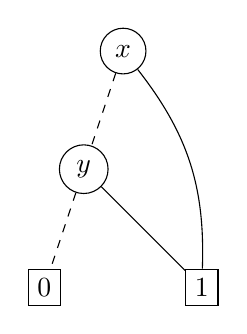
\begin{tikzpicture}


	\node[circle, draw] (x) at (0, 3){$x$};
	\node[circle, draw] (y) at (-0.5, 1.5) {$y$};
	\node[rectangle, draw] (0) at (-1, 0) {0};
	\node[rectangle, draw] (1) at (1, 0) {1};

	\draw (x) -- (y)[dashed];
	\draw (x) to[bend left=20] (1);
	\draw (y) to (0)[dashed];
	\draw (y) to (1);
\end{tikzpicture}
\qquad\quad 
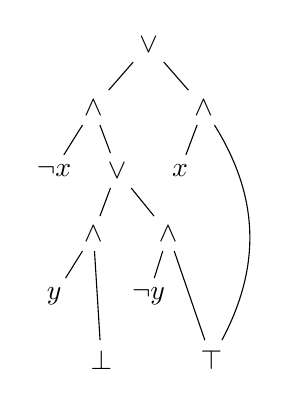
\begin{tikzpicture}
  \node (o1) at (0, 4) {$\lor$};
  \node (a1) at (-0.7, 3.20) {$\land$};
  \node (a2) at (0.7, 3.20) {$\land$};
  \node (x1) at (-1.2, 2.40) {$\lnot x$};
  \node (o2) at (-0.4, 2.40) {$\lor$};
  \node (x2) at (0.4, 2.40) {$x$};
  \node (a3) at (-0.7, 1.60) {$\land$};
  \node (a4) at (0.25, 1.60){$\land$};
  \node (y2) at (0, 0.8) {$\lnot y$};
  \node (y1) at (-1.2, 0.8) {$y$};
  \node (0) at (-0.6, 0){$\bot$};
  \node (1) at (0.8, 0){$\top$};

	\draw (o1) to (a1);
	\draw (o1) to (a2);
	\draw (a1) to (x1);
	\draw (a1) to (o2);
	\draw (a2) to (x2);
	\draw (a2) to[bend left=30] (1);
	\draw (o2) to (a3);
	\draw (o2) to (a4);
	\draw (a3) to (y1);
	\draw (a3) to (0);
	\draw (a4) to (y2);
	\draw (a4) to (1);

	
\end{tikzpicture}

	\caption{An OBDD (left) and the corresponding NNF sentence (right). Although the former seems much more compact, the difference in size is only linear and both representations are essentially the same.}
\label{nnf_obdd}

\end{figure}
 
 This ``knowledge compilation map" was the starting point for this project. Taking into account the various criteria for suitable representations described above, we searched the literature aiming to find a good candidate to replace BDDs. 

After considering a number of different representations including tree-of-BDDs \cite{trees_of_bdds}, BDD-trees \cite{bdd_trees}, and several other subsets of NNF described in \cite{compilation_map}, we opted for a relatively novel target compilation language called \textit{sentential decision diagram} (SDD). 

SDDs are a subset of NNF, and they satisfy essential properties such as succintness and polynomial-time Boolean operations. Also, they had not yet been experimented with in the context of symbolic model checking, for state-space representation. 
Moreover, some of the experimental results presented in \cite{sdd_1} and \cite{sdd_3} demonstrate that SDDs can lead to a significant improvement on BDDs in terms of computation time and memory usage. 

In the next section we present SDDs in full details, delaying our own experimental results to the following chapters.


\section{Sentential Decision Diagrams}

Most of the content in that section is taken from the work of A. Darwiche in \cite{sdd_1}, the first paper written on SDDs. 

\subsection{Preliminaries}

To define SDDs formally we must start with some preliminary definitions and results related to Boolean functions. 

\begin{definition} 
We say that a function $f$ \textit{essentially depends} on a variable $x$ iff $f|_{x} \neq f|_{\lnot x}$, and we write $f(X)$ if $f$ essentially depends on variables in $X$ only.
If $f(Z)$ is a function, we also write $f(X, Y)$ when $X$, $Y$ are sets forming a partition of $Z$.
\end{definition}
The following definition is the basis for the construction of SDDs:

\begin{definition} (Decompositions and partitions)
An \textit{($X$,$Y$)-decomposition} of a function $f(X, Y)$ is a set of pairs $\{(p_1, s_1),...,(p_n, s_n)\}$ such that $$ f = (p_1(X) \land s_1(Y)) \lor ... \lor (p_n(X) \land s_n(Y)).$$
The decomposition is said to be \textit{strongly deterministic} on $X$ if $p_i(X) \land p_j(X) = \bot$ for $i \neq j$. In this case, each ordered pair $(p_i, s_i)$ in the decomposition is called an \textit{element}, each $p_i$ a \textit{prime} and each $s_i$ a \textit{sub}.

Let $\alpha = \{(p_1, s_1),...,(p_n, s_n)\}$ be an ($X,Y$)-decomposition, and suppose $\alpha$ is strongly deterministic on $X$.
Then $\alpha$ is called an $X$-\textit{partition} iff its primes form a partition (i.e primes are pairwise mutually exclusive, each prime is consistent, and the disjunction of all primes is valid).
We say that $\alpha$ is \textit{compressed} if $s_i \neq s_j$ for $i \neq j$.
\end{definition}

\begin{example} 
Let $f(x, y, z) = (x \land y) \lor (x \land z)$. Then $\alpha = \{(x, y\lor z)\}$ is an $(\{x\}, \{y, z\})$-decomposition of $f$ which is strongly deterministic (as there is only one prime). It is however not an $\{x\}$-partition, but $\beta = \{(x, y\lor z), (\lnot x, \bot)\}$ is, since $x, \lnot x$ form a partition. Note that $\beta$ is compressed. 
\end{example}

\noindent Remark that in an $X$-partition $\bot$ can never be prime, and if $\top$ is prime then it is the only prime. Moreover primes determine subs, so two $X$-partitions are different iff they contain distinct primes.

\begin{theorem}
\label{theorem_apply}
Let $\circ$ be a Boolean operator and let $\{(p_1, s_1),...,(p_n, s_n)\}$ and $\{(q_1, r_1),...,(q_m, r_m)\}$  be $X$-partitions of Boolean functions $f(X, Y)$ and $g(X, Y)$ respectively. Then $$\{(p_i \land q_j, s_i \circ r_j) \mid  p_i \land q_j  \neq \bot \}$$ is an $X$-partition of $f \circ g$.
\end{theorem}
\begin{proof}
 Since $p_1, ..., p_n$ and $q_1, ..., q_m$ are partitions, the $(p_i \land q_j)$ also form a partition for $i = 1, ..., n$, $j = 1, ..., m$ and $p_i \land q_j \neq \bot$. So the given decomposition is an $X$-partition of some function.

Consider now an instantiation \textbf{z} of variables $X\cup Y$, so \textbf{z} consists of an instantiation \textbf{x} of $X$, and an instantiation \textbf{y} of $Y$. 
Then, since $\{p_k\}$ and $\{q_l\}$ are partitions, there must exist a unique $i$ and a unique $j$ such that $\textbf{x} \models p_i$ and $\textbf{x} \models q_j$, i.e $p_i(\textbf{x}) = q_j(\textbf{x}) = \top$. Then $f(\textbf{x}, \textbf{y}) = s_i(\textbf{y})$ and $g(\textbf{x}, \textbf{y}) = r_j(\textbf{y})$, so $(f\circ g)(\textbf{x}, \textbf{y}) = s_i(\textbf{y})\circ r_j(\textbf{y}).$

Evaluating the given decomposition at instantiation \textbf{z} also gives $s_i(\textbf{y}) \circ r_j(\textbf{y})$, hence result. 
\end{proof}

As we see later on, an important consequence of Theorem~\ref{theorem_apply} is the polynomial time operations available on SDDs. Canonicity of SDDs is due to the following result:

\begin{theorem}
\label{unique_compressed}
A function $f(X, Y)$ has exaclty one compressed $X$-partition.
\end{theorem}
\begin{proof}
Let $\textbf{x}_1, ..., \textbf{x}_k$ be \textit{all} instantiations of variables $X$. Then $\{(\textbf{x}_1, f|_{\textbf{x}_1}), ..., (\textbf{x}_k, f|_{\textbf{x}_k})\}$ is an $X$-partition of $f$. Let $s_1, ..., s_n$ be the distinct elements of $f|_{\textbf{x}_1}, ..., f|_{\textbf{x}_k}$, and for each $s_i$ define $p_i = \bigvee_{f|_{\textbf{x}_j} = s_i} \textbf{x}_j$.
Then $\alpha = \{(p_1, s_1), ..., (p_n, s_n)\}$ is a compressed $X$-partition of $f$. 

Suppose now that $\beta = \{(q_1, r_1), ..., (q_m, r_m)\}$ is another compressed $X$-partition of $f$. Then $\alpha$ and $\beta$ must have different partitions, i.e. $\{p_i\} \neq \{q_j\}$. Since they are both \textit{partitions}, there must exist a prime $p_i$ of $\alpha$ which overlaps with two different primes $q_j$ and $q_k$ of $\beta$, i.e. there exist distinct instantiations \textbf{x}, \textbf{x}' of $X$ such that $\textbf{x} \models p_i \land q_j$ and $\textbf{x}' \models p_i \land q_k$. Then we have $f|_\textbf{x} = \alpha_\textbf{x} = s_i = r_j = \beta_\textbf{x}$, and $f|_\textbf{x'} = \alpha_\textbf{x'} = s_i = r_k = \beta_\textbf{x'}$. So $r_j = r_k$, a contradiction as $\beta$ is compressed.  
\end{proof}

\subsubsection{Vtrees}

Vtrees (for ``variable trees") are to SDDs what variable orders are to BDDs. A vtree completely determines the structure of an SDD, so they are crucial to the viability of SDDs in practice.

\begin{definition}
A \textit{vtree} for variables $X$ is a full binary tree whose leaves are in one-to-one correspondence with the  variables in $X$. We will often not distinguish between a vtree node $v$ and the subtree rooted at $v$, and the left and right children of a node $v$ will be denoted $v^l$ and $v^r$, respectively.
\end{definition}

\begin{figure}
\centering
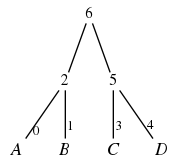
\includegraphics[scale=0.5]{balancedABCD.png}
\qquad
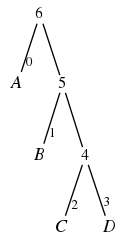
\includegraphics[scale=0.5]{rightlinearABCD.png}


\caption{Two vtrees for $X = \{A, B, C, D\}$, both inducing the order $[A, B, C, D]$.}
\label{fig:vtree_examples} 

\end{figure}
Each vtree \textit{induces} a variable order, namely the order in which leaves are visited during a left-right traversal of the vtree. Note that a vtree on a set $X$ is stronger than a total order of the variables in $X$, as two different vtrees may induce the same order; an example is shown in Figure~\ref{fig:vtree_examples}.

\subsection{Definition and Construction}

The construction of an SDD for a Boolean function $f$ with respect to a vtree $v$ is done by a recursive algorithm on the children nodes of $v$. 

Let $v$ be the vtree on the left of Figure~\ref{fig:vtree_examples}, and let $$f(A, B, C, D) = (A \land B) \lor (B \land C) \lor (C \land D).$$

The decomposition of $f$ at the vtree node $v$ goes as follows: we split the variables in $X$ into two subsets by separating variables in $v^l$ from those in $v^r$: we obtain $\{A, B\}$ and $\{C, D\}$. We compute the unique compressed $\{A, B\}$-partition $\alpha$ of $f$:
\begin{align*}
f(A, B, C, D) &= (A \land B) \lor (B \land C) \lor (C \land D)\\
&= ((A \land B) \land \top) \lor ((\lnot A \land B) \land C) \lor (\lnot B \land (C \land D)).
\end{align*}
So $\alpha = \{(\lnot B , C\land D), (\lnot A \land B, C), (A \land B, \top)\}$. The next step is to decompose the primes of $\alpha$ with respect to $v^l$, and its subs with respect to $v^r$. 
The vtree node $v^l$ splits the set $\{A, B\}$ into two subsets $\{A\}$ and $\{B\}$, so the non-trivial primes of $f$, namely $A \land B$ and $\lnot A \land B$ have SDDs $\{(A,B), (\lnot A, 
\bot)\}$ and $\{(\lnot A, B), (A, \bot)\}$, respectively. Similarly, we compute a $\{C\}$-partition of the only non-trivial sub of $f$, namely $C \land D$, and get $\{(C, D), (\lnot C, \bot)\}$, which is also an SDD since all its elements are constants or literals. 
The resulting SDD for $f$ is
$$\{(\lnot B , \{(C, D), (\lnot C, \bot)\}), (\{(\lnot A, B), (A, \bot)\}, C), (\{(A, B), (\lnot A, \bot)\}, \top)\},$$
which is very hard to read. But SDDs are generally written in their graphical representation, as shown below.

\subsubsection{Graphical Representation of SDDs}

The SDD constructed for function $f$ is represented on the left in Figure~\ref{fig:sddexample1}. On the right is the SDD for $f$ constructed with respect to the vtree on the right in Figure~\ref{fig:vtree_examples}.

A decomposition is represented by a circle with outgoing edges pointing to its elements, and an element is represented by a pair of boxes where the left box represents the prime and the right box represents the sub. If one of them is another decomposition, we leave the box empty and draw an edge pointing to the circle node representing it.

\begin{figure}
\centering
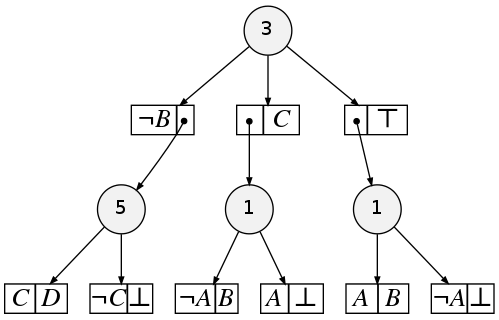
\includegraphics[scale=0.3]{balancedfirstexample.png}
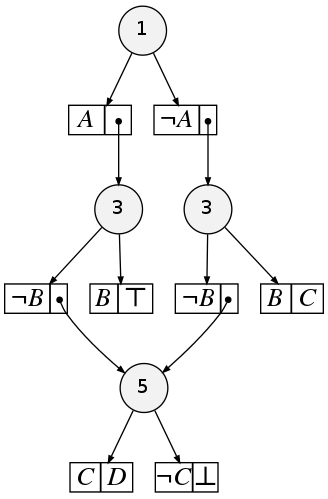
\includegraphics[scale=0.3]{rightlinearfirstexample.png}

\caption{SDDs for $f = (A \land B) \lor (B \land C) \lor (C \land D)$ corresponding to the vtrees in Figure~\ref{fig:vtree_examples}. Notice that identical SDD nodes have been merged.}
\label{fig:sddexample1} 
\end{figure}

The next two definitions formally define the syntax and semantics of SDDs.

\begin{definition} (Syntax) Let $v$ be a vtree. $\alpha$ is an SDD that respects $v$ iff: 
\begin{itemize} 
\item $\alpha = \top$ or $\alpha = \bot$
\item $\alpha = X$ or $\alpha = \lnot X$, and $v$ is a leaf with variable $X$
\item $v$ is an internal node (i.e. it has children), and $\alpha$ is a partition  $\{(p_1, s_1), ..., (p_n, s_n)\}$ such that for all $i$, $p_i$ is an SDD that respects $v^l$ and $s_i$ is an SDD that respects $v^r$.
\end{itemize}
In the first two cases we say that $\alpha$ is \textit{terminal}, and in the third case $\alpha$ is called a \textit{decomposition}. For SDDs $\alpha$ and $\beta$, we write $\alpha = \beta$ iff they are \textit{syntactically equal}.
\end{definition}

\begin{definition} (Semantics)
Let $\alpha$ be an SDD. We use $\langle . \rangle$ to denote the mapping from SDDs to Boolean functions, and we define it inductively as follows: 
\begin{itemize} 
\item $\langle \top \rangle = \top$ and  $\langle \bot \rangle = \bot$
\item $\langle X \rangle = X$ and $\langle \lnot X \rangle = \lnot X$, for all variables $X$
\item $\langle\{(p_1, s_1), ..., (p_n, s_n)\}\rangle = \bigvee_{i = 1}^n \langle p_i \rangle \land \langle s_i \rangle  $
\end{itemize}
We say two SDDs $\alpha$ and $\beta$ are \textit{equivalent} (written $\alpha \equiv \beta$) if $\langle \alpha \rangle = \langle \beta \rangle$.

\end{definition}

\subsection{Canonicity and Operations} 

It is obvious that if SDDs $\alpha$ and $\beta$ are equal, then they are equivalent. We would however like 
to impose conditions on the construction of $\alpha$ and $\beta$  so that $\alpha \equiv \beta \Rightarrow \alpha = \beta$, which would make SDDs a \textit{canonical }representation, a crucial property.
We begin with a few definitions and lemmas.

\begin{definition}
Let $f$ be a non-trivial Boolean function. We say $f$ \textit{essentially depends} on vtree node $v$ if $v$ is a deepest node that includes all variables that $f$ essentially depends on. 
\end{definition}

\begin{lemma}
A non-trivial function essentially depends on exactly one vtree node.
\label{unique_vtree_function}
\end{lemma} 
 
\begin{definition}
An SDD is \textit{compressed} iff all its decompositions are compressed. It is \textit{trimmed} iff it does not have decompositions of the form $\{(\top, \alpha)\}$ or $\{(\alpha, \top), (\lnot\alpha, \bot)\}$ for some SDD $\alpha$.
\end{definition}


These two properties are very accessible. An SDD is compressed as long as all $X$-partitions used during its construction are compressed, and it can be trimmed by traversing it bottom-up and replacing decompositions of the form  $\{(\top, \alpha)\}$ or $\{(\alpha, \top), (\lnot\alpha, \bot)\}$ by $\alpha$. 
Theorem~\ref{canonicity} below shows that they are in fact sufficient for the representation to be canonical. To prove it we first need another lemma. 

\begin{lemma}
Suppose $\alpha$ is a non-trivial, compressed and trimmed SDD. Then $\alpha$ respects a unique vtree node $v$, which is the unique node that the Boolean function $f = \langle \alpha \rangle$ essentially depends on.
\label{unique_vtree_sdd}
\end{lemma}

\begin{theorem} 
\label{canonicity}
Let $\alpha$ and $\beta$ be compressed and trimmed SDDs. Then $$\alpha = \beta \Leftrightarrow \alpha \equiv \beta.$$
\end{theorem}

\begin{proof}
$(\Rightarrow)$ is clear. For $(\Leftarrow)$, suppose that $\alpha \equiv \beta$ and let $f = \langle \alpha \rangle = \langle \beta \rangle.$ If $f$ is constant, then $\alpha$ and $\beta$ are trivial SDDs, therefore they are equal.
Suppose  now that $f$ is non-trivial, and let $v$ be the vtree node that $f$ essentially depends on (it is unique by Lemma~\ref{unique_vtree_function}). Then by Lemma~\ref{unique_vtree_sdd}, $\alpha$ and $\beta$ respect $v$. 
We continue the proof by structural induction on $v$. 

If $v$ is a leaf, then $\alpha$ and $\beta$ are terminals. But $f$ is non-trivial so $\alpha$ and $\beta$ are equivalent literals, and so they must be equal. 
Suppose now that $v$ is internal, and that the theorem holds for $v^l$ and $v^r$. Let $X$ be the variables in $v^l$ and $Y$ be the variables in $v^r$. 
Write $\alpha = \{(p_1,s_1), ..., (p_n,s_n)\}$  and $\beta = \{(q_1,r_1), ..., (q_m,r_m)\}$, where the $p_i, q_j$ are SDDs with respect to $v^l$ and the $s_i, r_j$ are SDDs with respect to $v^r$. Then  $\{(\langle p_1 \rangle,\langle s_1\rangle), ..., (\langle p_n\rangle,\langle s_n\rangle)\}$ and  $\{(\langle q_1 \rangle,\langle r_1\rangle), ..., (\langle q_n\rangle,\langle r_n\rangle)\}$ are $X$-partitions of $f$, and they are compressed since $\alpha$ and $\beta$ are compressed SDDs. So by Theorem~\ref{unique_compressed}, they are the same. So $n = m$, and for all $i$ we have $\langle p_i\rangle = \langle q_i \rangle $ and $\langle s_i \rangle = \langle r_i\rangle$, possibly after reordering. Then by definition $p_i \equiv q_i$ and $s_i \equiv r_i$, which by induction implies that $p_i = q_i$ and $s_i = r_i$. So $\alpha = \beta$.
\end{proof}

\subsubsection{Operations on SDDs} 

We start right away by giving the pseudo-code for the \texttt{apply} algorithm on SDDs, which combines two SDDs $\alpha$ and $\beta$ using a Boolean operator $\circ$, provided they respect the same vtree node.

\label{operations}
 \begin{figure}
 
\begin{lstlisting}[mathescape]

 1 function apply($\alpha$, $\beta$, $\circ$)
 2  if $\alpha$ and $\beta$ are constants or literals
 3    return $\alpha \circ \beta$   
 4  else if cache($\alpha$, $\beta$, $\circ$) != null
 5    return cache($\alpha$, $\beta$, $\circ$)
 6  else
 7    $\gamma$ = {}
 8    for all elements ($p_i$, $s_i$) in $\alpha$
 9      for all elements ($q_j$, $r_j$) in $\beta$ 
10        $p$ = apply($p_i$, $q_j$, $\land$)
11        if p != $\bot$
12          $s$ = apply($s_i$, $r_j$, $\circ$)
13          if $\nexists$ element ($q$, $s$) in $\gamma$
14            add ($p$, $s$) to $\gamma$
15          else 
16            add (apply($p$, $q$, $\lor$), s) to $\gamma$
17          end if
18        end if
19      end for
20    end for
21    return cache($\alpha$, $\beta$, $\circ$) = $\gamma$
22  end if
23 end function
$$
\end{lstlisting}
 \end{figure}


If $\alpha$ and $\beta$ are compressed, then this algorithm returns a compressed SDD for $\alpha \circ \beta$. 
Theorem~\ref{theorem_apply} ensures that \texttt{apply($\alpha$, $\beta$, $\circ$)} is in fact an SDD, while the if condition on line 13 checks that its subs are distinct, thereby making it a compressed SDD. The use of the \texttt{cache} in the pseudo-code emphasises the fact that any implementation of \texttt{apply} could be significantly improved by keeping the set of computed SDDs in a cache in memory. 

If lines 13 - 16 were replaced by \texttt{add ($p$, $s$) to $\gamma$} (i.e. if we omitted the code checking that the obtained SDD is compressed), the time complexity of \texttt{apply} on SDDs $\alpha$ and $\beta$ would be $O(|\alpha||\beta|)$ and all Boolean operations could be done in polynomial time. 
The additional recursive call on line 16 makes the algorithm harder to analyze, considering \texttt{p} and \texttt{q} are not part of either $\alpha$ or $\beta$. In practice however, this additional call makes \texttt{apply} much more efficient since it is then dealing with compressed SDDs, easier to manipulate \cite{sdd_1}. 

The other SDD operation which will be essential for symbolic model checking is \texttt{condition}, which computes the conditioning of an SDD on a literal. 
Although \cite{sdd_1} doesn't supply pseudo-code for \texttt{condition}, it can be done in polynomial time.
Let $\alpha$ be an SDD for function $f$, and let \textbf{x} be a literal; The SDD for function $f|_{\textbf{x}}$, i.e. the result of \texttt{condition(\textbf{x}, $\alpha$)} can be obtained by applying the following operations, bottom-up:
\begin{itemize}
\item For each element $(\beta, \textbf{x})$ of $\alpha$, we replace it with $(\beta, \top)$ if no other element has $\top$ as a sub, or by $(\texttt{apply($\beta$, $\gamma$, $\lor$}), \top)$ if $(\gamma, \top)$ was another element with sub $\top$. In the latter case we also remove the element $(\gamma, \top)$ and direct all its incoming edges to the newly created node. (Note that $\gamma$ would have been unique, since $\alpha$ is compressed).

\item For each element $(\beta, \lnot\textbf{x})$ of $\alpha$ we do the same as the above, replacing $\top$ with $\bot$.

\item For each element $(\textbf{x}, \beta)$ of $\alpha$, we replace the partition of which it is an element with $\beta$, essentially ``removing one level" of this particular SDD.

\item We remove each element  $(\lnot\textbf{x}, \beta)$ of $\alpha$. Note that the remaining decomposition will still be an $X$-partition for some set $X$, since the previous steps will have been applied on the rest of the elements.
\end{itemize}
Observe that although this can be done in polynomial time, the \texttt{condition} operation on SDD is slightly more time-consuming than the equivalent on BDDs, which simply involves removing each node labelled ($\lnot$)\textbf{x}, redirecting its incoming edges to the corresponding child. 


\subsection{OBDDs are SDDs}
\label{bdds_are_sdds}
To end the background section of this report, we would like to  focus on the fact that \textit{OBDDs are SDDs}, i.e. if we regard them as subsets of NNF, then OBDD $\subseteq$ SDD. We first give a simple explanation for why this is the case. 

Consider an SDD $\alpha$ respecting a vtree $v$ such that every left child is a leaf. Such a vtree is said to be \textit{right-linear}, and every decomposition in $\alpha$ will be of the form $\{(A, \beta_1), (\lnot A, \beta_2)\}$ for some variable $A$ and SDDs $\beta_1, \beta_2$. 
But this is the same decomposition as that occuring in a BDD at the node labelled with $A$.

Suppose now that $B$ is a BDD for function $f$, and that $v$ is the \textit{only} right-linear vtree inducing the variable order for $B$. Then the SDD for $f$ respecting $v$ is \textit{syntactically equal} to $B$, when both are regarded as NNF sentences. Hence there is a one-to-one correspondence between BDDs and SDDs respecting right-linear vtrees. 
Figure~\ref{fig:bdds_are_sdds} illustrate this with an example. 

\begin{figure}
\centering
\begin{subfigure}{.5\textwidth}
\centering
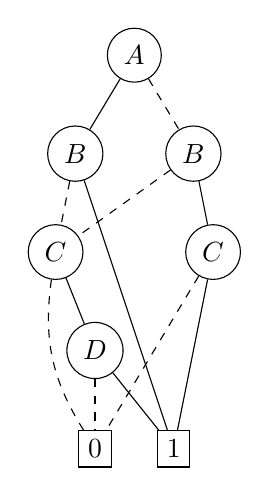
\begin{tikzpicture}

\node[draw] (0) at (2, 0) {0};
\node[draw] (1) at (3, 0) {1};
\node[draw, circle] (A) at (2.5, 5) {$A$};
\node[draw, circle] (B1) at (1.75, 3.75) {$B$};
\node[draw, circle] (B2) at (3.25, 3.75) {$B$};
\node[draw, circle] (C1) at (1.5, 2.5) {$C$};
\node[draw, circle] (C2) at (3.5, 2.5) {$C$};
\node[draw, circle] (D) at (2, 1.25) {$D$};

\draw (D) to (0)[dashed];
\draw (D) to (1);
\draw (A) -- (B1);
\draw (A) -- (B2)[dashed];
\draw (B1) -- (C1)[dashed];
\draw (B2) -- (C1)[dashed];
\draw (B1) -- (1);
\draw (B2) -- (C2);
\draw (C1) to[bend right=20] (0)[dashed];
\draw (C1) -- (D);
\draw (C2) to (0)[dashed];
\draw (C2) -- (1);


\end{tikzpicture}
\end{subfigure}%
\begin{subfigure}{.5\textwidth}
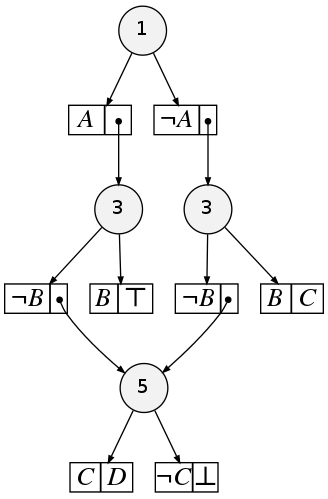
\includegraphics[scale=0.35]{rightlinearfirstexample.png}
\end{subfigure}
\caption{The BDD for  $f = (A \land B) \lor (B \land C) \lor (C \land D)$ with variable order $[A, B, C, D]$ (left), and the SDD respecting the right-linear vtree inducing the same order (right). Note that this is the vtree depicted on the right of Figure \ref{fig:vtree_examples}.}
\label{fig:bdds_are_sdds}

\end{figure}

A very general consequence of this is that any application of BDDs in computer science could be implemented using SDDs instead, as it would retain the attractive properties of BDDs while benefiting from the potential reduction in size that SDDs present. In the more specific case of this project, we will see in a later chapter that this correspondence was extremely useful in helping us compare the efficiency of SDDs with that of BDDs in model checking: by restricting our SDD implementation to right-linear vtrees, we were able to compare both programs more accurately by taking into account the overhead due to the difference in \textit{implementation} (as opposed to a difference in size between the two structures -- we knew these were the same!).

\chapter{A First Model Checker Based on SDDs}

For the first time, SDDs are being used for symbolic model checking. Implementing a model checker based on SDDs therefore required some prior reflection.
In this chapter, we start by presenting the existing code base and libraries which our implementation relies upon (Sections \ref{sdd_package} \& 
\ref{mcmas}). Using these ``tools", we consider our options, and devise a theoretical approach which will guide the implementation of our model checker, as well as our evaluation strategy in the next chapter (\ref{3.3}).
Finally, we describe the design, algorithms, and challenges of our implementation (\ref{implementation} to \ref{issues}).

\section{Preliminary I: The SDD Package}
\label{sdd_package}

\subsection{Overview}

\textit{The SDD Package} \cite{SDD_website} is a C library which can be used to create and manipulate SDDs. It was developed at UCLA by the Automated Reasoning group, who first introduced SDDs. Its current version is 1.1.1.  


The SDD Package API contains most of the functions required for the use of SDDs in model checking. This includes basic manipulations such as conjunction, disjunction, and negation of Boolean functions represented by SDDs, conditioning a function on a literal, and quantifying out variables (the SDD equivalent of $\exists$ and $\forall$). Additionally, the API makes possible a number of operations on vtrees, including \textit{rotating }and \textit{swapping} (these are crucial for navigating the space of vtrees in the context of SDD minimisation, see below for details). 

The \textit{SDD manager} is the focal point for all the SDD operations in the program. It is there to ensure that all SDDs in the program have been built with respect to the same vtree, and it handles SDD conversions in the case of a vtree modification. It also gives the user access to a number of statistics, helpful for tracking a program's memory usage or the size of some SDD nodes. 

\subsection{Standard Vtrees}
\label{std_vtrees}

Four different ``classes" of vtrees are pre-implemented in the SDD package, i.e. can be created in one function call, provided a variable order is supplied. 
They are:
\begin{itemize}
\item right-linear: all left children are leaves
\item left-linear: all right children are leaves
\item balanced: the vtree is a balanced binary tree, i.e. both children of a node have the same number of leaves (if total number is even)
\item vertical: every node has a leaf child, which is alternatively the right child or the left child
\end{itemize}
Throughout this report we refer to these as the \textit{standard} vtrees. An example of each is given in Figure~\ref{fig:std_vtrees_example}.

\begin{figure}
\centering
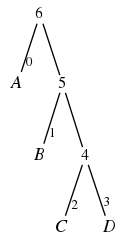
\includegraphics[scale=0.4]{rightlinearABCD.png}
\quad
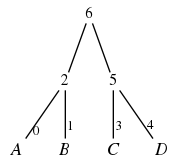
\includegraphics[scale=0.4]{balancedABCD.png}
\quad
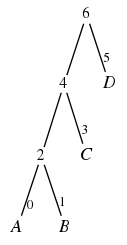
\includegraphics[scale=0.4]{leftlinearABCD.png}
\quad
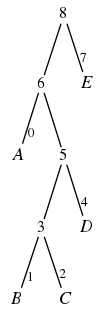
\includegraphics[scale=0.4]{verticalABCDE.png}
\caption{The four standard vtrees, in order: right-linear, balanced, left-linear, and vertical.}
\label{fig:std_vtrees_example}
\end{figure}

\subsection{Dynamic SDD Minimisation}
\label{sdd_dao_algo}
One particularly important feature of the SDD Package is \textit{dynamic SDD minimisation}. When enabled, this feature automatically attempts to minimise the size of a manager's SDD nodes by searching for a better vtree. Unfortunately this is not always a more efficient solution as searching the space of vtrees is a very lengthy process: there are $\frac{(2n -2)!}{(n-1)!}$ distinct vtrees over $n$ variables!

An vtree search algorithm was proposed in \cite{sdd_3} for more efficient dynamic minimisation of SDDs. This algorithm relies on three standard binary tree operations: left-rotation, right-rotation, and swap; these operations can be applied on any node of a vtree, and they are sufficient for navigating the space of all vtrees \cite{knuth}. They are implemented in the SDD Package as \texttt{swap\_vnode()}, \texttt{lr\_vnode()}, and \texttt{rr\_vnode()}. Figure~\ref{fig:vtree_operations} shows in what way these operations affect vtrees.
\begin{figure}
\centering
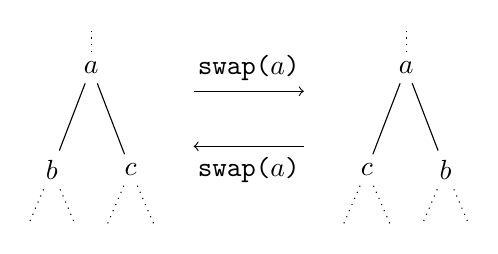
\begin{tikzpicture}
\node (a1) at (0, 0) {$a$};
\node (b1) at (-0.5, -1.3) {$b$};
\node (c1) at (0.5, -1.3) {$c$};
\node (a2) at (4, 0) {$a$};
\node (b2) at (3.5, -1.3) {$c$};
\node (c2) at (4.5, -1.3) {$b$};

\draw (a1) to (b1);
\draw (a1) to (c1);
\draw (a1) to (0, 0.5)[dotted];
\draw (b1) to (-0.8, -2)[dotted];
\draw (b1) to (-0.2, -2)[dotted];
\draw (c1) to (0.2, -2)[dotted];
\draw (c1) to (0.8, -2)[dotted];

\draw (a2) to (b2);
\draw (a2) to (c2);
\draw (a2) to (4, 0.5)[dotted];
\draw (b2) to (3.2, -2)[dotted];
\draw (b2) to (3.8, -2)[dotted];
\draw (c2) to (4.2, -2)[dotted];
\draw (c2) to (4.8, -2)[dotted];

\draw (1.3, -0.3) to (2.7, -0.3) [->, =<latex];
\draw (2.7, -1) to (1.3, -1) [->, =<latex];
\node (s1) at (2, 0) {\texttt{swap(}$a$\texttt{)}};
\node (s2) at (2, -1.3) {\texttt{swap(}$a$\texttt{)}};


\end{tikzpicture}
\\
\begin{tikzpicture}
\node (0) at (0, 1) {};
\node (a1) at (0, 0) {$a$};
\node (b1) at (-0.5, -1.3) {$b$};
\node (c1) at (0.5, -1.3) {$c$};
\node (d1) at (-1.1, -2.6) {$d$};
\node (e1) at (-0.1, -2.6) {$e$};
\node (a2) at (4, 0) {$b$};
\node (b2) at (3.5, -1.3) {$d$};
\node (c2) at (4.5, -1.3) {$a$};
\node (d2) at (3.9, -2.6) {$e$};
\node (e2) at (4.9, -2.6) {$c$};

\draw (a1) to (b1);
\draw (a1) to (c1);
\draw (a1) to (0, 0.5)[dotted];
\draw (b1) to (d1);
\draw (b1) to (e1);
\draw (d1) to (-1.4, -3.3)[dotted];
\draw (d1) to (-0.8, -3.3)[dotted];
\draw (e1) to (-0.4, -3.3)[dotted];
\draw (e1) to (0.2, -3.3)[dotted];
\draw (c1) to (0.2, -2)[dotted];
\draw (c1) to (0.8, -2)[dotted];


\draw (a2) to (b2);
\draw (a2) to (c2);
\draw (a2) to (4, 0.5)[dotted];
\draw (c2) to (d2);
\draw (c2) to (e2);
\draw (d2) to (3.6, -3.3)[dotted];
\draw (d2) to (4.2, -3.3)[dotted];
\draw (e2) to (4.6, -3.3)[dotted];
\draw (e2) to (5.2, -3.3)[dotted];
\draw (b2) to (3.2, -2)[dotted];
\draw (b2) to (3.8, -2)[dotted];

\draw (1.3, -0.8) to (2.7, -0.8) [->, =<latex];
\draw (2.7, -1.5) to (1.3, -1.5) [->, =<latex];
\node (s1) at (2, -0.5) {\texttt{rr(}$a$\texttt{)}};
\node (s2) at (2, -1.8) {\texttt{lr(}$a$\texttt{)}};


\end{tikzpicture}
\caption{The main vtree operations and their effect.}
\label{fig:vtree_operations}
\end{figure}



We now give an informal description of the algorithm in \cite{sdd_3} (the one implemented in the SDD Package). We start with a vtree node $v$ (typically, the current vtree of the manager). The algorithm first makes two recursive calls on the children of $v$, ensuring that their structure is optimal. Suppose that the vtree obtained is the one represented below:

\begin{tikzpicture}

\node (0) at (-1, 0.8) {};
\node (0) at (-1, -3.6) {};

\node (v) at (5, 0) {$v$};
\node (b) at (4.2, -1.3) {$x$};
\node (c) at (5.8, -1.3) {$y$};
\node (d) at (3.6, -2.6) {$a$};
\node (e) at (4.6, -2.6) {$b$};
\node (f) at (5.4, -2.6) {$c$};
\node (g) at (6.4, -2.6) {$d$};


\draw (v) to (b);
\draw (v) to (c);
\draw (v) to (5, 0.5)[dotted];
\draw (b) to (d);
\draw (b) to (e);
\draw (d) to (3.3, -3.3)[dotted];
\draw (d) to (3.9, -3.3)[dotted];
\draw (e) to (4.3, -3.3)[dotted];
\draw (e) to (4.9, -3.3)[dotted];
\draw (f) to (5.1, -3.3)[dotted];
\draw (f) to (5.7, -3.3)[dotted];
\draw (g) to (6.1, -3.3)[dotted];
\draw (g) to (6.7, -3.3)[dotted];

\draw (c) to (f);
\draw (c) to (g);

\end{tikzpicture}


Then, the algorithm considers two vtree \textit{fragments} of $v$, the \textit{l-vtree} and the \textit{r-vtree}. The l-vtree is the binary tree with leaves $a, b$ and $y$, and the r-vtree is the binary tree with leaves $x, c$ and $d$. The algorithm attempts to compute the 24 distinct vtree fragments obtained by applying rotations and swaps to the l- and r-vtrees, and then selects the one leading to the most effective reduction in size for the SDD nodes depending on $v$. 


For each of the three vtree operations, users of the SDD package can set limits on the time needed to compute them, and the increase in size that they induce; this means that not all 24 vtree fragments above are necessarily computed. 

\subsection{Comparison with CUDD}
\label{comparison_with_cudd}

CUDD is the C$++$ BDD library used by MCMAS (see below) for BDD manipulation, and it is therefore our reference for all practical comparisons between SDDs and BDDs. 

Here we simply give an account of the differences between  CUDD and the SDD package, in order for our comparisons to be fair: we are interested in the relative efficiency of the data structures, not the packages, and therefore it is important that we take into account any differences in design and implementation. 

Fortunately, the libraries have a very similar flavour. For instance both are organised around a manager handling all internal operations. A few differences are worth mentioning:
\begin{itemize}
\item Both libraries have an automated garbage collection feature, and both are based on node reference counts. However the SDD Package requires users to manually increment and decrement the reference counts of each SDD node they create, whereas in CUDD this is optional (MCMAS doesn't use it). 
\item In the SDD Package the automated garbage collection and dynamic minimisation features are not independent, i.e. one cannot be enabled without the other being too. This means that when experimenting with SDDs without dynamic minimization, we find that a lot of unused nodes are kept in memory, sometimes preventing the program from generating any more SDDs in an efficient way (once the memory has run out, which happens relatively often in model checking when no garbage collection takes place). This is not the case in CUDD. 
\item An important difference in implementation is in the way the libraries handle existential quantification (the function $\exists$). We devote an entire subsection to this issue (\ref{exist_implementation}).

\end{itemize}
\label{gc}

\section{Preliminary II: MCMAS} 
\label{mcmas}

MCMAS (Model Checker for Multi-Agent Systems) is a BDD-based model checker written in C$++$, which was developed, and is currently maintained at Imperial College in the Verification of Autonomous Systems group. It was specifically designed for the verification of multi-agent systems, and users can write system descriptions in a language called ISPL (Interpreted System Programming Language), whose syntax is very much inspired from the definition of interpreted systems (\ref{IS}). MCMAS is able to verify CTLK formulae, and a recent version also incorporates ATL (the Alternating-Time Temporal Logic \cite{atl}, not discussed here), however it does not support the verification of LTL(K) formulae.

In order to better understand the implementation of the model checker, the reader is strongly advised to start by getting an overview of the main components in an ISPL file. For this purpose we supply a full example of a simple interpreted system encoded in ISPL: the \textit{Bit Transmission Problem}, available in Appendix~\ref{BTP}. ISPL is a fairly straightforward language, we therefore will not spend any more time describing it here, but should anything remain unclear, the reader is refered the MCMAS User Manual \cite{MCMAS_website}.



The model checker built for this project is (for a large part) based on the MCMAS code base. In this section we outline some of the MCMAS internal implementation details in order to help the reader understand the steps undertaken when replacing BDDs with SDDs. Moreover, MCMAS will be the basis of our BDDs/SDDs comparisons in the next chapter so it is important for the reader to understand the different configuration options.

\subsection{Important Classes and Methods}
\label{MCMAS_steps}
The ISPL parser in MCMAS creates a model of the system using the following important classes: 
\begin{itemize}
\item \texttt{basic\_agent}: an agent in the system, consisting of a protocol, an evolution, a set of variables and a set of actions
\item \texttt{evolution\_line} and \texttt{protocol\_line}: a line in the evolution or in the protocol of an agent, consisting of a Boolean expression and an assignment or (respectively) an action
\item \texttt{bool\_expression} and \texttt{assignment}
\item \texttt{variable}, \texttt{basic\_type}, \texttt{int\_value}, \texttt{enum\_value}, \texttt{bool\_value},  \texttt{rangedint}, \texttt{atomic\_proposition}, \texttt{laction}: agent variables, their types and their values
\item \texttt{modal\_formula}: a CTLK formula to be checked in the model.
\end{itemize}
Throughout the model checking procedure the \textit{BDD parameters} are carried by the program and passed as argument to the various methods. They are encapsulated in a structure (\texttt{struct bdd\_parameters}) and contain all the important data required by the algorithm, in particular: 
\begin{itemize}
\item three vectors \texttt{v}, \texttt{pv}, and \texttt{a}, containing the Boolean variables used in the model for encoding states, next states, and actions respectively
\item a vector \texttt{vRT}, containing for each agent the BDD for its transition relation 
\item the BDD \texttt{in\_st} representing the set of initial states, and (once computed) the BDD \texttt{reach} for the reachable state space
\item a pointer to the BDD cache
\item a vector \texttt{is\_formulae} containing the \texttt{modal\_formula} objects for each CTLK formula to check
\end{itemize}
MCMAS is (quite literally) an implementation of the model checking algorithm described in \ref{explicit}. However, as a symbolic model checker it also contains procedures for encoding protocols, transition relations, sets of states and actions, etc., and in fact these constitute a very large part of the code. 
We list the main steps in the execution of the program:
\begin{enumerate}
\item Parse ISPL file, allocate variables and set up CUDD (see \ref{variable_allocation} below)
\item Compute the BDD for the global transition relation
\item Compute the BDD for the reachable state space 
\item For each modal formula $\varphi$, compute
\texttt{SAT($\varphi$)} and check that it is a subset of $I$
\item Output result and free memory
\end{enumerate}


\subsection{Variable Allocation}
\label{variable_allocation}
Variable allocation is the process of allocating manager variables (created with the manager) to agents and determining the various sets of variables needed for symbolic representation within each agent: state variables, primed state variables (a copy of the state variables representing the \textit{next }states), and action variables.

For each agent, MCMAS first computes the number of variables needed in each of the aforementioned sets by calls to the functions \texttt{state\_BDD\_length()} and \texttt{action\_BDD\_length()}.

The \texttt{basic\_agent} functions \texttt{allocate\_BDD\_2\_variables()} and \texttt{allocate\_BDD\_2\_actions()} are then used for variable allocation: they assign a portion of both \texttt{v} and \texttt{a} to each agent, giving them start and end \textit{indices}. Note that this forces all of an agent's state variables (and similarly, action variables) to be next to each other in \texttt{v} (and similarly, \texttt{a}). 

It may seem confusing that variable allocation happens before the user has been able to select a particular variable order, but in fact no actual variables have yet been allocated, only their position in the arrays. The user's choice will then affect the way the \textit{manager}'s variables are dispatched across \texttt{a}, \texttt{v}, and \texttt{pv}. 

In MCMAS, the user can choose between four \textit{standard} different variable orders. We take the time to present them here, not only because of the impact that this choice has on the overall performance, but also for reference in the future chapters (where we compare these orders with various SDD vtrees).

\subsection{Standard Variable Orders}
 \label{std_orderings}
Suppose MCMAS is running on an example requiring $n$ state variables denoted $x_1, ..., x_n$, and $m$ action variables denoted $a_1, ..., a_m$. By definition there are $n$ primed state variables (the next state is a state, so it can be represented with the $n$ state variables), these are denoted $x_1', ..., x_n'$. 
Suppose also that there are $k$ agents, and that for each $i$, agent $i$ has been allocated variables $x_{i_1}, ..., x_{i_{n_i}}$, $x_{i_1}', ..., x_{i_{n_i}}'$ and $a_{j_1}, ..., a_{j_{m_i}}$, for some $n_i, m_i \in \mathbb{N}$ and where $i_1, ..., i_{n_i}$ and $j_i, ..., j_{m_i}$ are sequences of consecutive integers.



The manager will then have $2n + m$ variables in total, and the following are the possible four ordering options with respect to which BDDs will be constructed throughout the process.
In options 2 to 4, variables are ordered using the agent order, so that we get an ordering of the form $$ [\mbox{variables for agent } 1, \mbox{variables for agent } 2, ...,  \mbox{variables for agent } k],$$ 
and the difference lies in the way variables are ordered within each agent set.
\begin{itemize}
\item Ordering option 1 (no interest in agent allocation):
$$[x_1, ..., x_n, x_1', ..., x_n', a_1, ..., a_m]$$
\item Ordering option 2 (variables for agent $i$):
$$
 [x_{i_1}, x_{i_1}', x_{i_2}, x_{i_2}',..., x_{i_{n_i}}, x_{i_{n_1}}', a_{i_1}, ..., a_{i_{m_1}}]
$$
\item Ordering option 3 (variables for agent $i$):
$$
 [x_{i_1}, ..., x_{i_{n_i}},a_{i_1}, ..., a_{i_{m_1}}, x_{i_1}', ..., x_{i_{n_1}}']
$$
\item Ordering option 4 (variables for agent $i$):
$$
 [x_{i_1}, ..., x_{i_{n_i}}, x_{i_1}', ..., x_{i_{n_1}}', a_{i_1}, ..., a_{i_{m_1}}]
$$
\end{itemize}

These different orderings can have a great impact on the size of the resulting BDD, and consequently on MCMAS computation times. It is generally accepted that the ordering option 2 is the best to use in model checking multi-agent systems. It is based on the concept of \textit{variable interleaving} in OBDDs \cite{interleaving}, and adapted to agents.


\subsection{Algebraic Decision Diagrams}
\label{algebraic_decision_diagrams}

MCMAS supports bounded integer variables (e.g. \texttt{x : 0..3}), and allows Boolean conditions to be numeric identities (e.g. \texttt{(x > 2)} or \texttt{(x + y = 3)} for integer vars \texttt{x} and \texttt{y}). 

If an agent has an integer variable with a large range of values, then the number of Boolean variables needed to represent its state is also large (if variable \texttt{x} has $n$ possible values, the corresponding agent needs at least $\log_2(n)$ state variables). 

To avoid this, MCMAS uses alternative data structures called \textit{algebraic decision diagrams} (ADD, \cite{add}) to represent these variables and expressions. The CUDD manager also handles ADDs, and the ADD variables needed are stored in global vectors \texttt{addv} and \texttt{addpv}.

As there is no SDD equivalent for ADDs (yet!), our model checker does not support examples containing numerical values and expressions.
Note that all these examples \textit{could} technically be implemented in ISPL so that our model checker supports them, by simply replacing an integer range by an \textit{enum} containing all the possible values that the variable can take: for example 
$$\texttt{x : 0..3} $$
could be declared as $$\texttt{x : \{zero, one, two, three\}}$$
and expressions such as $$\texttt{if (x > 1)}$$ could be translated to $$\texttt{if (x = two) or (x = three)}.$$
With ADDs being beyond the scope of this project, we did not study them further (in particular we did not look into the ADD reduction done by CUDD in the background), and therefore thought better not to implement this to keep the comparison fair between MCMAS and our model checker. 

\section{Model Checking with Sentential Decision Diagrams}
\label{3.3}
In this section, we discuss the feasibility of implementing a model checker based on SDDs and the choices involved. We also reflect on the \textit{potential }that SDDs have to outperform BDDs, and we explore from a theoretical point of view the different ways of using them.

\subsection{Suitability of SDDs for Model Cheking}

SDDs are representations of Boolean functions, and as such, they can theoretically be used to represent state spaces and transition relations of a model. We have seen in the background section of this report that there exist polynomial-time algorithms for Boolean operations (AND, OR, NOT) on SDDs, as well as for conditioning an SDD on a literal, both of these being \textit{essential} to an efficient model checker implementation. We showed also that these two operations (generally refered to in this report as \texttt{apply} and \texttt{condition}) are sufficient for implementing the entire model checking algorithm defined in \ref{explicit}. Hence, the SDD data structure is \textit{a priori} a suitable representation for symbolic model checking, and its early success \cite{sdd_3} in knowledge compilation gives us hope that it might even constitute an improvement on BDDs. 

One of the directions of our investigation will be to search the space of vtrees in order to compare them, and give a first assessment of some specific vtree constructions in terms of their efficiency in the context of model checking. Before we launch into this search, we start by analysing \textit{theoretically} the impact that the vtree will have on the overall performance of the model checker. This should give us some insights into how to structure this search, which would otherwise be very unpromising considering the size of the space of vtrees.

\subsection{The Importance of Vtrees} 

We have seen that the size of an SDD can be significantly affected by the vtree with respect to which is is constructed. But in addition, the vtree has a huge impact on the efficiency of some SDD operations such as \texttt{apply} or \texttt{condition}. 

In particular, a characteristic of a vtree $v$ that we will look at very carefully is the size and configuration of its \textit{left subtrees}, by which we mean the left children of the nodes of $v$, and their descendents.	This is not a formally defined vtree characteristic, but it is of fundamental importance to the suitability of a particular vtree for model checking. 

Recall the construction of an SDD for function $f$ with respect to a vtree $v$. It involves creating an $X$-partition of $f$, where $X$ is the set of variables in $v^l$. If $X$ contains a lot of the variables in $f$, the \textit{primes} of $f$ will be large. But in SDDs, primes are given more importance than subs, as shown for example in the \texttt{apply} algorithm in \ref{operations}, where the recursive call on subs is only made if the recursive call on corresponding primes did not return $\bot$.

The search for a good vtree does \textit{not }amount to reducing primes as much as possible: if this were the case, there would be absolutely no point in trying to replace BDDs (whose \textit{primes} are as small as possible -- they are just one literal!) with SDDs. But the ultimate objective of vtree optimisation is to construct primes in such a way that: \begin{itemize}
\item The number of decisions to make is less than it would be in a BDD;
\item Decisions remain quick enough.
\end{itemize}
The word ``decision" is deliberately used in a vague sense here, to incorporate both the combination of two SDD elements in an execution of \texttt{apply}, or the evaluation of an SDD on a variable instantiation (for \texttt{condition}).

\subsection{A New Perspective on Vtrees}
\label{new_perspective}
Taking into account the fact that the efficiency of a vtree fundamentally depends on the composition of its left children, we introduce a more precise way of describing vtrees which emphasises this point and facilitates our explanations in the rest of this report. Recall first that for a vtree node $v$, its left and right children are respectively refered to as $v^l$ and $v^r$. By slight abuse of notation, we write $v^{r^2}$ for the right child of the right child of $v$, etc.

\begin{definition} Let $v$ be a vtree. An \textit{l-subtree} of $v$ is an element of the sequence $$v^l, (v^r)^l, (v^{r^2})^l, ..., (v^{r^{k-1}})^l, v^{r^k},$$ where $k \geq 0$ is the smallest integer such that $(v^{r^{k+1}})$ is a leaf.
\end{definition}

An example is given in Figure~\ref{fig:lsubtrees_vtree_example}. Observe that for a right-linear vtree $v$, l-subtrees of $v$ are all leaves (expect for the last one which is a node with two leaves). Also, if $v$ is left-linear or vertical, the only l-subtree of $v$ is $v$ itself (we set $v^{r^0} = v$). 

\begin{figure}
\centering
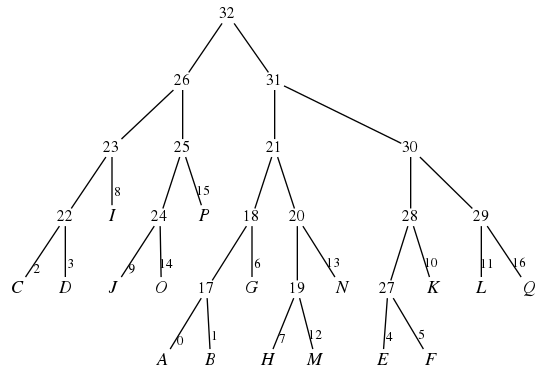
\includegraphics[scale=0.5]{pseudorightlinearfirstexample.png}
\caption{The l-subtrees of this vtree are the subtrees rooted at nodes 26, 21, 28, and 29.}
\label{fig:lsubtrees_vtree_example}
\end{figure}

We also want to emphasise the fact that each variable of $v$ lies on one of its l-subtrees, and furthermore, the sets of variables induced by the l-subtrees form a partition of the set of variables of $v$.

Our ``new perspective" on a vtree consists in identifying it using the partition of the variables that its l-subtrees induces. That is, from now on we will be \textit{comparing }vtrees by comparing their l-subtrees, and we will be \textit{constructing }vtrees by creating a partition of the variable set, which will be used as a basis for constructing l-subtrees that we can then arrange and link together.

\subsection{Vtree Options in Practice}
\label{vtree_options_in_practice}
The formalism defined in the previous section will facilitate the task of exploring the space of vtrees for applications to model checking, as we can now more easily characterise ``good" vtrees. In practice however, whatever these good vtrees turn out to be, we need to be able to \textit{generate} them automatically from a model of the multi-agent system we wish to verify. This means that this characterisation needs to have some \textit{meaningful} links to the model itself (as a random partition is unlikely to do the job well, and doesn't constitute a very good heuristic!).

Recall that during the encoding process of an interpreted system for a multi-agent system, we assign a set of variables to each agent, separated into state variables, ``primed" state variables, and action variables. This gives us a \textit{natural} splitting of the full set of variables, made up of three different sets for each agent.

We now have a wide range of easily generated, meaningful options to investigate, as a variable partition can lead to a lot of different vtrees: we can change the shape of the l-subtrees we create from it, their order, or even combine them, split them further, etc. These options will be thoroughly explored in the Evaluation chapter of this report. 

\subsection{Dynamic Minimisation in Symbolic Model Checking}
\label{dynamic_with_sdds}
Dynamic minimisation is an essential element to symbolic model checking in practice. When state spaces grow larger, model checking without dynamic minimisation is often very impractical. 

In \ref{sdd_dao_algo}, we described the dynamic vtree search algorithm implemented in the SDD Package, which our model checker relies upon. Recall that this algorithm automatically searches through the \textit{whole} space of vtrees, i.e. it may lead to a complete re-structuring of the vtree if it improves the size of the SDDs considered. Although this might be a very good option for knowledge compilation, where the goal is to find the most compact representation possible, it seems to be a considerable effort in symbolic model checking, where a large number of different SDDs will be used at the same time (by the same \textit{manager}), and modified a lot within a short period of time.

For this reason, we introduce the idea of limiting this automatic search to only \textit{some} vtrees. The main option we will look at consists in re-structuring the l-subtrees only. It seems that this would constitute a faster search (as far less vtrees will be considered), while retaining the potential advantage which was originally brought by the particular choice of l-subtrees. So far this is of course just an idea, and we will need to either demonstrate, or reject this idea using real-life examples.

\section{Implementation Specifics}
\label{implementation}

\subsection{Adapting MCMAS}

We implemented a model checker for multi-agent systems entirely based on SDDs for symbolic representations. 

Our starting point was the MCMAS source code, in which we proceeded to replace every call to CUDD with equivalent calls to the SDD Package. Throughout, we managed the reference counts of our SDD nodes by calls to \texttt{sdd\_ref()} and 
\texttt{sdd\_deref()}. Note that this often requires the introduction of temporary nodes; specifically, this occurs when updating the value of a node based on its previous value. For instance, the CUDD statement 
\begin{verbatim}
// f, g are BDDs
f = f * g; 
\end{verbatim}
setting the value of $f$ to be the conjunction of the BDDs for $f$ and $g$, becomes
\begin{verbatim}
// f, g are SddNode*
SddNode* tmp;
f = sdd_conjoin(tmp = f, g, manager);
sdd_ref(f, manager);
sdd_deref(tmp, manager);
sdd_deref(g, manager); // (if this is the last time we use g)
\end{verbatim}
This is to ensure that the previous SDD node pointed to by $f$, which the code can no longer access, is garbage collected. As a more complete example we provide the code for the \texttt{compute\_reach()} function in appendix (To Do).

The main steps of our model checker are the same as those of MCMAS described in \ref{MCMAS_steps}, and therefore the important functions which had to be adapted for SDDs are: 
\begin{itemize}
\item the functions \texttt{encode\_protocol()}  and \texttt{encode\_evolution()} for each agent, used to compute the global transition relation
\item the \texttt{compute\_reach()} function for computing the SDD representing the global reachable state space
\item the \texttt{check\_formula()} method (the implementation of \texttt{SAT})
\end{itemize}

Additionally, new data types and functions had to be defined in order to deal with the SDD-specific aspects of the program. We replaced the MCMAS BDD parameters by our own \textit{SDD parameters} (see appendix) containing the results of the variable allocation process in three different vectors: \texttt{variable\_sdds}, \texttt{primed\_variable\_sdds}, \texttt{action\_variable\_sdds}.

\subsection{Existential Quantification}
\label{exist_implementation}

Recall  (\ref{exist}) that the model checking algorithm relies on the functions $\mbox{pre}_\exists$ and $\mbox{pre}_\forall$, which themselves depend on existential quantification, or the process of relaxing the constraint on one or more variables in a function. 

In CUDD, the function responsible for existential variable quantification is \texttt{Cudd\_bddExistAbstract()}. This takes as input two BDDs $f$ and $c$, and returns the BDD for $f$ after existential quantification of all variables in $c$. The implementation of this function is based on the following recursive algorithm called \texttt{restrict}, originally described in \cite{unified_framework}: 
\begin{figure}

\begin{lstlisting}[mathescape]

function restrict(f, c):
// pre:$ \mbox{ c != } \bot$ and variables of c are all variables of f
  if c = $\top$ or f = $\bot$ or f = $\top$
    return f
  x := top variable in f // the root of the BDD
  if (x = top variable in c)  
    return (restrict(f$|_{\mbox{x}}$, c$|_{\mbox{x}}$) $\lor$ restrict(f$|_{\lnot\mbox{x}}$, c$|_{\mbox{x}}$))
  else // x does not appear in c
    return (x $\land$ restrict(f$|_{\mbox{x}}$ , c)) $\lor$ ($\lnot$x $\land$ restrict(f$|_{\lnot\mbox{x}}$ , c))
end
$\\$
\end{lstlisting}
\end{figure}


In the context of symbolic model checking, existential quantification of a set of variable $X$ from a function $f$ can be done in CUDD by a call to \texttt{Cudd\_bddExistAbstract(f, c)}, where \texttt{f} is the BDD for $f$ and \texttt{c} is a function essentially depending on all the variables in $X$ (in MCMAS \texttt{c} is set to be the conjunction of all the variables in $X$).

In the SDD Package, existential quantification can only be done one variable at a time, by calling \texttt{sdd\_exists(x, f, manager)} which returns $\exists x f$. Our first solution was to iteratively call this function on every variable in $X$, but our first experiments revealed that this method was very slow. We therefore implemented the above algorithm in our model checker as an attempt to reduce computation time:
\begin{figure}

\begin{lstlisting}[mathescape]

SddNode* restrict_sdd(SddNode* f, SddNode* c, SddManager* manager) 
{
  if(sdd_node_is_false(c)) // not allowed
    return NULL; 
  if(sdd_node_is_true(c) || sdd_node_is_false(f) || sdd_node_is_true(f))
    return f;
  SddLiteral x = get_top_variable(f);
  SddLiteral y = get_top_variable(c);
  if (x == y) {
    SddNode* res1 = restrict_sdd(sdd_condition(x, f, manager), sdd_condition(x, c, manager), manager);
    SddNode* res2 = restrict_sdd(sdd_condition(-x, f, manager), sdd_condition(x, c, manager), manager);
    return sdd_disjoin(res1, res2, manager);
  } else {
    SddNode* res1 = restrict_sdd(sdd_condition(x, f, manager), c, manager);
    SddNode* res2 = restrict_sdd(sdd_condition(-x, f, manager), c, manager);
    return ite(sdd_manager_literal(x, manager), res1, res2, manager);
  }
}

\end{lstlisting}
\caption*{}
\end{figure}
In the code above, we have omitted the calls to \texttt{sdd\_ref()} and \texttt{sdd\_deref()} for clarity. Also, \texttt{ite} refers to an implementation of the ITE (If-Then-Else) operator on Boolean functions, namely $$\mbox{ITE}(f, g, h) = (f \land g) \lor (\lnot f \land h).$$

Another point worth discussing is the notion of ``top variable" for an SDD. In a BDD, this is unambiguously refering to the variable with which the root is labelled, and this choice of variable for the start of the algorithm is clearly induced by the conditioning algorithm on BDDs, which consists in removing the \textit{false} outcoming edge for each node labelled with the variable in question -- if this is the top variable, then this amounts to simply removing the right (or left) subtree of the BDD. 

In an SDD however, this is not so obvious. It would make sense for the ``top variable" of a vtree to correspond to the top variable in the variable order induced by that vtree. In that case, it would be in that same order that the variables of \texttt{c} would be existentially quantified from $f$ in our implementation.

But looking at the algorithm for \texttt{condition} described in \ref{operations} (which we \textit{assume} the SDD Package uses, or at least a similar version), it is unclear what order would be the most efficient. (TODO say that we try both?)


\section{SDD-Specific Features}

\subsection{Vtrees and Variable Orders}

Recall that in the SDD Package, the use of the standard vtrees is only possible when a variable order is supplied. For convenience, we implemented the four standard MCMAS variable orders in our model checker, for use with one of the standard vtree, thereby making 16 different vtrees available. These orderings are implemented within the \texttt{get\_var\_order()} function, whose code is documented in appendix. 

As previously mentioned, being able to create our own ``non-standard" vtrees will be crucial for the utility of the project.  
The SDD Package API is lacking some basic functions in that area, most probably because it is generally sufficient for users to rely on the standard vtrees, together with the dynamic minimisation feature. There are, for example, no ways of constructing a vtree bottom-up, as one would construct an SDD node. Hence, to create our own customised vtrees, we had the following two options:
\begin{itemize}
\item Generate a variable order to create one of the standard vtrees, and apply swaps, left- and right-rotations until the vtree obtained is the desired vtree
\item Generate a \textit{vtree format} text file and use \texttt{sdd\_vtree\_read()} to create a \texttt{Vtree} object. According to the SDD manual, this file format is normally used to save vtrees to file in order to re-use them in the future. The function \texttt{sdd\_vtree\_save\_to\_file()} is the way to generate the file from an existing vtree.

\end{itemize}
We chose the second option, simply because it seemed more convenient than computing the set of operations to apply to get from one vtree to another. The vtree format, without being particularly readable, has the advantage of being relatively simple in syntax and therefore easy to generate. 

The API of the SDD Package was clearly not designed to edit and manipulate vtrees practically, so as a replacement we created a new tree structure, the \texttt{vtree\_node}, defined thus: 
\begin{verbatim}
struct vtree_node 
{
  // the children
  vtree_node * left; 
  vtree_node * right;
  // more data for file generation
  int size;
  bool isleaf;
  int id;
};
\end{verbatim}

This very simple structure significantly facilitated the process of constructing vtrees. We could simply create a leaf \texttt{vtree\_node} for each variable needed, and construct the vtree bottom-up. Observe that the variables themselves are not stored; this is because we organise the nodes so that each variable is \textit{one more} than the ID of the leaf which contains it (IDs start from 0 in the file, whereas variables are numbered from 1 in the SDD manager).

 The function \texttt{vtree\_node\_get\_file\_content()} was written to recursively return the string representing the \texttt{vtree\_node} in the file format required by \texttt{sdd\_vtree\_read()}. The code for the function, as well as an example, can be found in the appendix (To do). 

In practical applications, the number of variables is not known in advance but we still need a way of generating the vtree dynamically. To this aim, we wrote the \texttt{create\_vtree()} function which is called in the program as soon as the number of variables needed is known, but \textit{before} the SDD manager is created, so that the vtree produced can be used during its initialisation -- note that this is only possible since our vtree is not based on actual variables but on a temporary structure which does not involve the manager. 

To use \texttt{create\_vtree()}, we need to pass it the number of variables that the vtree should consist of, as well as the desired \textit{vtree type}. This is an integer corresponding to one of the various vtrees which we implemented: vtree types 1-4 correspond to the standard vtrees defined in \ref{std_vtrees}, whereas types 4-8 are ``new" vtrees which we used for experimentation, thinking they had more potential in the context of model checking. We leave out the details for now and use the evaluation section to describe these various vtrees and the corresponding experimental results.

\subsection{A New Dynamic Vtree Search Algorithm}
\label{dynamic_with_sdds_implementation}

In \ref{dynamic_with_sdds}, we introduced the idea of a new dynamic vtree search algorithm, focusing on a re-structuring of the l-subtrees only. In this subsection we describe our implementation of this new algorithm.


First note that in the SDD Package, the default implementation of the minimisation function can be modified using \texttt{sdd\_manager\_set\_minimize\_function()},  indicating which function should be used instead.
The code for our replacement function is as follows: 
\begin{figure}

\begin{lstlisting} [mathescape]
Vtree* vtree_group_minimize(Vtree* vtree, SddManager* manager) {
  // start from the root   
  Vtree* current = vtree; 
  // repeat until a leaf is reached
  while (!sdd_vtree_is_leaf(sdd_vtree_right(current))) {
    // minimise the left subtree using original algorithm
    sdd_vtree_minimize(sdd_vtree_left(current), manager);
    // and go down one step to the right
    current = sdd_vtree_right(current);	
  }
  sdd_vtree_minimize(current);
  return vtree;
} 
\end{lstlisting}

\end{figure}

To illustrate this, we refer the reader to the vtree in Figure~\ref{fig:lsubtrees_vtree_example} above. If called on this vtree, the \texttt{vtree\_group\_minimize()} function will \textit{only }search for an improvement of the subtrees rooted at nodes 26, 21, 28 and 29 (i.e. the l-subtrees). 

\section{Software Engineering Issues}
\label{issues}
Here we explain some of the challenges faced during the implementation of the model checker, as well as our approach to testing correctness of the model checker. 

\subsection{Garbage Collection}

As described in \ref{gc}, the SDD Package has a automatic garbage collection feature based on reference counts, but it leaves the referencing and dereferencing of nodes to the user. 

If not done properly, node referencing can lead to issues such as unwanted garbage collection, dead nodes kept in memory, or dead node dereferencing, all of which being very undesirable (but for different reasons).

This forced the constant track-keeping of node reference counts and required more debugging time. Nonetheless, it is important to mention that the manual referencing and dereferencing of nodes is probably more efficient in the long run than if the SDD manager had to do it in the background, which would require more thinking on its part.

\subsection{Comparing SDDs and BDDs}

The goal of this implementation was to build an SDD-based model checker which produced the same results as MCMAS in all circumstances. We needed to make sure that the Boolean functions representating our sets of states and transition relations were the same at each step of our model checking algorithm. Unfortunately, there is no convenient and precise way of programmatically comparing an SDD with a BDD. 

The only \textit{exact} method available is to look at the Boolean function corresponding to each data structure, and compare these. However, due to their syntactic differences, it had to be done using a SAT checker (we used \cite{minisat}), which is a good solution for small functions but becomes impractical very quickly when the number of variable exceeds about 20 (which happens in all non-trivial cases).  

An useful alternative is to construct the SDD with respect to a right-linear vtree and the BDD with the equivalent variable ordering (see \ref{bdds_are_sdds} for details), to ensure that the resulting structures are comparable. We then have two options:
\begin{itemize}

\item Compare the graphical representation of each data structure, provided by both APIs via a DOT file \cite{dot}. An image is often enough to tell if two representations are not equivalent, but in the case where they are, it can be a very long process to manually verify it.
\item Compare the size (i.e. the number of nodes) of each structure. Again, most of the time two non-equivalent representations have very different sizes, but representations with comparable sizes are not necessarily equivalent (note that due to the way SDD and BDD nodes are counted, the size of a BDD is not exactly the same as the size of the equivalent SDD so this method is not 100\% conclusive either).

\end{itemize}
 This second option is nonetheless the only available solution in the case of very large SDDs and BDDs, which explains the difficulty in debugging larger examples.

Reflecting back on this issue, it would have been much less time-consuming to write a small logic equivalence tool ensuring that the Boolean functions obtained from two equivalent data structures was not only equivalent, but also \textit{syntactically equal}, to reduce the problem to a simple comparison of strings. We did not anticipate enough the amount of work that would be required when debugging the model checker.

\subsection{Correctness}

 Due to the reasons mentioned above, we had to use a few simple tricks to make sure that our code was indeed an implementation of the model checking algorithm. 

The first technique we used was that of comparing the \textit{output} of our model checker with that of MCMAS, on the set of examples that we had available (see \ref{ispl_examples} for a detailed description of these examples). Once we were certain that these were identical (so no obvious bugs existed), we did a more thorough search to ensure that there was nothing wrong with the code. 

Although our set of examples was relatively diverse, it certainly did not cover the whole range of expressions, data types, etc. available in ISPL, nor did it use the full set of CTLK connectives that ISPL supports.
Hence, our second approach to verification was to "invent" new formulae to check, using different combinations of connectives from those to be tested. Also, we made a series of modifications to the example ISPL files to check that most (not all, see \ref{algebraic_decision_diagrams}) of the ISPL syntax was handled by our model checker. This even revealed a bug in the MCMAS source code (which had persisted in our code) causing a segmentation fault when the input ISPL file used more than one bitwise XOR (\^{}). This bug has now been fixed (in both model checkers).

Although these verification techniques are not guaranteed to have caught all bugs, we are confident that they were sufficient for our purposes, and that in all the examples considered, both model checkers had the same outcome.


\chapter{Evaluation} 

\section{Introduction}

\subsection{Evaluation Strategy}

The objective of this evaluation is to experiment with SDDs in the context of model checking multi-agent systems, and explore the various in which situations our model checker performs best.

TODO 
 The plan for quantitative analysis is to do a side-by-side comparison of our model checker and MCMAS on a series of examples, and conclude. However, in order to provide a fair comparison we had to ensure that both structures were performing ``at the best of their abilities". 

There are suggested methods for the use of BDDs in model checking, in particular concerning initial variable orders~\cite{bdd_heuristics}. For the specific case of MCMAS we observe that the standard order number 2 (see \ref{std_orderings}) \textit{often} yields the best results.
On the other hand, SDDs had not yet been explored in the context of model checking, and consequently no heuristics existed. 

Through this evaluation we planned to remediate this by investigating various vtree constructions and comparing the resulting model checker with MCMAS. 

To start with, we decided to focus on the issue of \textit{static} vtree generation, for the situation where the vtree has to be determined \textit{before} SDDs are constructed, as opposed to continuously modified as the construction process happens -- this is called \textit{dynamic} minimisation. 

Although it may seem like wasted effort, the importance of static vtree generation is non-negligible, for two reasons: firstly, it helps us understand what aspects of the vtree have the greatest impact on the final SDD; secondly, even though dynamic minimisation is generally the most efficient technique, it can also be a very time-consuming process which some applications might find less practical. 

After this first investigation, we planned to look at the performance of SDDs when enabling the dynamic minimisation feature of the SDD Package, and compare it to BDD dynamic variable reordering as implemented in MCMAS.

We hoped that both of these analyses (static and dynamic) would provide enough information to know whether or not SDDs (as implemented in the SDD Package) are suitable for model checking multi-agent systems.

\subsection{Example Models}
\label{ispl_examples}

In this section, we describe the ``real-life" example models used as benchmarks throughout this chapter. This is to provide the reader with some context before launching into numerous tables of results, and to help understand the analysis we make of these results. 

Our set of examples is made up of three main classes of models, presented below. The (very trivial) bit transmission problem (Appendix~\ref{BTP}) is also sometimes used to demonstrate the \textit{inefficiency} of a particular technique, so we also provide some useful characteristics of this particular model. 

\subsubsection{The Dining Cryptographers}

The original dining cryprographers problem was introduced by D. Chaum in 1988, refering to the following situation: three cryptographers go out for dinner, and at the end of the meal, the waiter informs them that the bill has already been paid by someone, who could either be one of the cryptographers, or the National Security Agency (NSA). While respecting each other's right to remain anonymous, they would like to find out if the NSA has paid. They use the following two-step protocol: in the first step, each cryptographer flips a coin behind a menu, so that only them and the cryptographer to their right can see the outcome; then, they each know the outcome of two out of the three coin flips, and in the second step, the cryptographers that haven't paid publicly announce whether or not these two outcomes are the same. If one cryptographer \textit{has} paid for the meal, they announce the opposite. The NSA has paid for the meal only if there is an even number of "same". 

This problem can be generalised to any number $n$ of cryptographers, and modelled by a multi-agent system consisting of one agent for each cryptographer, and an environment holding information about the coin flipping outcomes and the cryptographers' claims.

With the help of an ISPL file generator, we use a \textit{parametrised} version of the dining cryptographers problem, allowing us to easily rescale the model depending on the efficiency of the approach considered. The CTLK formula we are verifying in this example is 
$$AG\left[(\mbox{odd} \land \lnot \mbox{c1paid}) \rightarrow (K_{c1} (\mbox{c2paid} \lor ... \lor \mbox{c$n$paid}) \land \lnot K_{c1} \mbox{c2paid} \land ...  \land \lnot K_{c1} \mbox{c$n$paid})\right],$$
which encodes the following true property:
\textit{ ``At any point, if we know that there is an odd number of `same' and the first cryptographer is not the one that paid for dinner, then the first cryptographer knows that one of the other cryptographers paid, without knowing which one''.}
\\\\

{\centering
\begin{tabular}{*{5}{c}}
\hline
\hline
\multicolumn{5}{c}{\textbf{Dining Cryptographers}}\\ \hline
$n$ & \#agents & \#reachable states & \#vars (states/actions) & depth \\\hline
4 & 5 (4 + env.) & 400  & 57 (24/9) & 4 \\ \hline
5 & 6 & 960  & 69 (29/11) & 4 \\ \hline
6 & 7 & 2240  & 81 (34/13) & 4 \\ \hline
7 & 8 & 5120  & 93 (39/15) & 4 \\ \hline
8 & 9 & 11520  & 105 (44/17) & 4 \\ \hline
9 & 10 & 25600  & 117 (49/19) & 4 \\\hline

\end{tabular}
\\}

\subsubsection{100 Prisoners and a Lightbulb}

The \textit{100 prisoners and a lightbulb} problem is a mathematical riddle. The problem, of unknown origin, is stated as follows:
\\\\
 \fbox{
\begin{minipage}{0.9\textwidth}
 \vspace{0.25cm}
One hundred prisoners have been newly ushered into prison. The warden tells them that starting tomorrow, each of them will be placed in an isolated cell, unable to communicate amongst each other. Each day, the warden will choose one of the prisoners uniformly at random with replacement, and place him in a central interrogation room containing only a light bulb with a toggle switch. The prisoner will be able to observe the current state of the light bulb. If he wishes, he can toggle the light bulb. He also has the option of announcing that he believes all prisoners have visited the interrogation room at some
point in time. If this announcement is true, then all prisoners are set free, but if it is false, all prisoners are executed. The warden leaves, and the prisoners huddle together to discuss their fate. Can they agree on a protocol that will guarantee their freedom? 
\vspace{0.2cm}
\end{minipage}
}
\\\\\\
There are several solutions to the riddle. The one that we will be verifying involves designating a ``counter" amongst the prisoners, who will be the only one allowed to announce whether he believes all prisoners have visited the room.

Using another file generator, we can create a parametrised (scalable) version of the problem as a multi-agent system, where the agents are the Prisoners (excluding the counter), the Counter, the Prison (keeping track of which prisoners have visited the room, and whether or not they have been released/executed), and the Environment (containing the current state of the light bulb and the identity of the prisoner being interrogated). The parameter $n$ corresponds to the number of prisoners, including the counter. We verify the following CTL properties: 
\begin{itemize}
\item $AF$ Release: \textit{The prisoners will eventually be released.} (False)
\item $EF$ Release: \textit{It is possible that the prisoners will eventually be released.} (True)
\item $EF$ Execute: \textit{It is possible that the prisoners will eventually be executed.} (False)
\item $AG \lnot\mbox{Execute}$: \textit{The prisoners will never be executed.} (True)
\end{itemize}
(It is a \textit{safe} model, in the sense that the counter will only make an announcement if he is absolutely certain that all prisoners have visited the room.)
\\\\

{\centering
\begin{tabular}{*{5}{c}}
\hline
\hline
\multicolumn{5}{c}{\textbf{Prisoners}}\\ \hline
$n$ & \#agents & \#reachable states & \#vars (states/actions) & depth \\\hline
3 & 5 (4 + env) & 50 & 33 (13/7) & 9 \\ \hline
5 & 7 & 746 & 50 (20/10) & 17 \\ \hline
6 & 8 & 2631 & 57 (23/11) & 21 \\ \hline
7 & 9 & 8980 & 64 (26/12) & 25 \\ \hline
8 & 10 & 30001 & 72 (29/14) & 29 \\ \hline
9 & 11 & 98798 & 81 (33/15) & 33 \\ \hline
10 & 12  & 322107 & 88 (36/16) & 37 \\ \hline
\end{tabular}
\\}
\subsubsection{The Needham-Schroeder Public-Key Protocol}

The Needham-Schroeder Public-Key protocol \cite{nspk} (NSPK) is a communication protocol based on public-key cryptography, aiming to establish mutual authentification between an initiator A and a responsor B.

As opposed to the previous two classes of models, this one is not parametrised, but we have different \textit{versions}, consisting in one or more \textit{instances} of the protocol. Each instance is an agent, and the environment stores information about each of them.

The CTLK formulae to check differ depending on the version, but all of them involve verifying that different instances of the protocol \textit{agree} by the time they are finished. For example, in the first version, the only formula to check is 
$$AG (\mbox{instance\_2\_end} \rightarrow K_{\mbox{instance\_2}}( \mbox{agree\_instance\_2\_and\_instance\_1})).$$
\\\\
{\centering
\begin{tabular}{*{5}{c}}
\hline
\hline
\multicolumn{5}{c}{\textbf{NSPK}}\\ \hline
version & \#agents & \#reachable states & \#vars (states/actions) & depth \\\hline
1 & 2 & 618 & 75 (29/17) & 6 \\ \hline
2 & 3 & 42240 & 107 (42/23) & 9 \\ \hline
4 & 3 & 5736 & 108 (42/24) & 6 \\ \hline
5 & 4 & $2.88\times10^6 $ & 176 (72/32) & 11 \\ \hline
6 &  & &  262(106/50) &  \\ \hline

\hline
\end{tabular}
\\}
\subsubsection{The Bit Transmission Problem}
The problem and its model are fully described in Appendix~\ref{BTP}. Below are some stats: \\

{\centering
\begin{tabular}{*{4}{c}}
\hline
\hline
\multicolumn{4}{c}{\textbf{Bit Transmission Problem}}\\ \hline
\#agents & \#reachable states & \#vars (states/actions) & depth \\\hline
3 & 18 & 17 (6/5) & 4 \\
\hline
\end{tabular}
\\}

\subsubsection{Range of Examples}

The dining cryptographers models are an example of a model where one of the agents (namely, the environment) has a very large evolution function, leading to an even larger local transition relation. The prisoners models are an example of a very \textit{deep} model, making it longer to obtain a fixed point in the reachable state space computation, and harder to check some of the formulae.
Finally, the NSPK are extremely large examples of models, particularly versions 5 and 6. 

These three ``classes" of models are therefore relatively diverse, very different from each other, and will help us analyse more accurately the results obtained in our experiments. 


\subsection{Experimental Framework} 

Throughout this chapter, we report a number of tables containing experimental results. Here, we attempt to describe as accurately as possible the framework in which these experiments took place, as well as the format in which we present the results. 

All benchmarks were run on a Linux Ubuntu 13.04 64-bit machine, with 16GB memory and a Intel Core i7-4770 processor at 3.40GHz. 
Results of all experiments are split into two tables: computation time and memory usage, where time measurements are in seconds, memory usage in megabytes. All computations were performed three times and computation times were averaged; the memory used is always the same on a particular example, as both MCMAS and our model checker are deterministic. In each table we indicate in bold the situations where SDDs outperformed BDDs.

We indicate by a dash `-' the cases where the system either ran out of memory, or reached a timeout of an hour. It is interesting to note that in the case of static vtree generation (4.2 \& 4.3), all dashes represent OOMs, whereas in our dynamic minimisation experiments (4.4), a dash always corresponds to a timeout.

For each situation explored, we selected a set of models from the ones described in \ref{ispl_examples}, including several of the same type with different parameters. This selection was done in such a way that the range of results would be as broad as possible, while remaining within the timeout/memory limit. 

Finally, in addition to the results of the experiments conducted on SDDs, most tables contain the best BDD results obtained on the same models, in order to make the comparison easier.

\section{Static Comparisons with Standard Vtrees}

We started our investigation by experimenting with the standard vtrees, namely right-linear, left-linear, balanced, and vertical. Recall that this first investigation was focused exclusively on static vtree generation, so we disabled \textit{both }the dynamic SDD minimisation feature in our model checker, and the CUDD dynamic reordering feature in MCMAS. Due to the SDD Package design, this forced the garbage collector to be off as well in our model checker.

\subsection{Right-Linear Vtrees} 

Our first experiments involved right-linear vtrees. Recall that BDDs are structurally identical to SDDs build using a right-linear vtree, and the same variable ordering (\ref{bdds_are_sdds}). Experimenting with this particular type of vtrees was therefore of significant importance, as it would allow us to compare both model checkers in the case where they were handling data structures of the exact same size.

\begin{table}
\centering
\begin{tabular}{|*{9}{c|}}
\hline
 & \multicolumn{2}{c|}{Ordering 1} & \multicolumn{2}{c|}{Ordering 2} & \multicolumn{2}{c|}{Ordering 3} & \multicolumn{2}{c|}{Ordering 4}\\
\cline{2-9}
& BDDs & SDDs & BDDs & SDDs & BDDs & SDDs & BDDs & SDDs\\ \hline
cryptos7 & 2.06 & 12.35 & 2.64 &  6.39 & 3.33 & 12.77 & 3.83 & 15.186 \\ \hline
cryptos8 & 11.85 & 56.02 & 17.24 & 30.42 & 20.41 & 58.70 & 23.85 & 69.54 \\ \hline
cryptos9 & 853.17 & \textbf{221.16} & 98.95 & 145.313 & 617.32 & \textbf{266.84} & 911.70 & \textbf{305.17} \\ \hline
pris9 & 50.14 & - & 11.47 & 252.21 & 12.52 & 369.83 & 17.31 & - \\ \hline
pris10 & 236.15 & - & 35.11 & - & 42.12 & -& 52.13 & -\\ \hline
nspk1 & 0.06 & 0.79 & 0.04 & 0.59 & 0.09 & 1.21 & 0.06 & 0.71 \\ \hline
nspk2 & 11.25 & 154.46 & 2.71 & 76.32 & 7.36 & 120.42 & 4.55& 84.15 \\ \hline
nspk4 & 1.29 & 27.29 & 0.32 & 9.79 & 1.75 & 23.74 & 0.95 & 14.68 \\ \hline
nspk5 & - & - & 158.62 & - & - & - & - & - \\ \hline
nspk6 & - & - & - &- & - & - & - & - \\ \hline
\end{tabular}
\\
\caption{Computation Time: SDDs were built with right-linear vtrees, and standard orderings}
\label{table:rightlineartime}
\vspace{1in}
\centering
\begin{tabular}{|*{9}{c|}}
\hline
 & \multicolumn{2}{c|}{Ordering 1} & \multicolumn{2}{c|}{Ordering 2} & \multicolumn{2}{c|}{Ordering 3} & \multicolumn{2}{c|}{Ordering 4}\\
\cline{2-9}
& BDDs & SDDs & BDDs & SDDs & BDDs & SDDs & BDDs & SDDs\\ \hline
cryptos7 & 198 & 782 & 160 & 306 & 248 & 656 & 272 & 791 \\ \hline
cryptos8 & 758 & 3120 & 647 & 1308 & 1024 & 2630 & 1120 & 3166  \\ \hline
cryptos9 & 3001 & 11556 & 2850 & 5566 & 4246 & 10134 & 4690 & 11927 \\ \hline
pris9 & 594 & - & 313 & 7658 & 3502 & 12382 & 4349 & -\\ \hline
pris10 & 1955 & - & 847 & - & 968 & - & 1218 & -\\ \hline
nspk1 & 16 & 34 & 13 & 24 & 25 & 50 & 17 & 34 \\ \hline
nspk2 & 324 & 2065 & 135 & 1012 & 493 & 1520 & 275 & 1104 \\ \hline
nspk4 & 92 & 624 & 45 & 223  & 188 & 693 & 81 & 344 \\ \hline
nspk5 & - & - & 3841 & - & - & - & - & -\\ \hline
nspk6 & -&- &- &-  &- &- &- &- \\ \hline
\end{tabular}
\\
\caption{Memory Usage: SDDs were built with right-linear vtrees, and standard orderings}
\label{table:rightlinearmemory}
\end{table}
 
Tables \ref{table:rightlineartime} and \ref{table:rightlinearmemory} correspond, respectively, to the time and memory comparisons of our model checker with MCMAS, when SDDs were built with right-linear vtrees. We include results for each of the four standard orderings with which the vtrees were constructed. 
\\\\
During this first phase of the investigation, it became quickly apparent that SDDs were \textit{not }better than BDDs in this particular situation, outperforming them top
in only three cases, and being slower in most cases, sometimes considerably (up to two orders of magnitude). The important difference in memory usage can be explained by the garbage collector being off in the SDD Package. 

We observe that the time difference is more important in the prisoners and NSPK examples than for the dining cryptographers. A particularity of these two examples is that they involve larger data structures: the prisoners models both have a large number of reachable states, and in the NSPK models, each agent is allocated around 40 variables, leading to very large transition relation SDDs.
These results therefore seem to imply that the SDD manager is not as efficient as CUDD when it comes to handling large data structures. We also mentioned that it was likely for the \texttt{condition} algorithm to be slightly more efficient on BDDs than on SDDs. 

These hypotheses are contradicted by the three situations where SDDs are faster than BDDs. We suspect that this is due a memory management issue in CUDD: it is possible that these particular models filled up the cache and slowed down the rest of the computation. This is difficult to check, as CUDD handles this internally. Moreover, pushing the comparison further would be impossible, as SDDs run out of memory at the next level. 

Although these particular results are disappointing, they could have been expected: although the data structures are equivalent, the SDD algorithms have not been particularly optimised for this particular type of vtrees, as they must be prepared to handle different types of data structures. On the other hand, CUDD was developped specifically for BDDs, and has the advantage of being much older and benefiting from the extensive BDD research done in the past few decades.  

To conclude this first subsection, we make the following remark: in this situation the model checkers are dealing with the \textit{exact} same structures, so these numbers \textit{should }be the same for BDDs and SDDs. But they aren't, for the reasons explained above and in \ref{comparison_with_cudd}. However, should the SDD Package ever become as efficient as CUDD, any improvement on the SDD numbers in Tables~\ref{table:rightlineartime} and \ref{table:rightlinearmemory} would be an improvement on BDDs. This is hypothetical, but it motivated the rest of our experiments, and in particular, the search for a better vtree.
\\\\
\textit{Note on BDD data: from now on, all the BDD data found in the comparison tables corresponds to computations using standard ordering number 2, the most efficient for BDDs in the vast majority of cases (\ref{std_orderings}).
}

\subsection{Other Standard Vtrees}

We moved on from right-linear vtrees, hoping that one of the other standard vtrees would lead to more efficient computations. This was not the case. 

\begin{table}
\centering
\begin{tabular}{|*{10}{c|}}
\hline
\multirow{2}{*}{} & \multirow{2}{*}{BDDs} & \multicolumn{4}{c|}{Left-Linear} & \multicolumn{4}{c|}{Vertical}\\ \cline{3-10}
& & O. 1 & O. 2 & O. 3 & O. 4  & O. 1 & O. 2 & O. 3 & O. 4 \\ \hline
btp & 0.02& 44.3 & 8.36 & 6.42 & 6.56 & 0.61 & 0.13 & 0.09 & 0.10 \\ \hline
cryptos4 & 0.02 & - & - & - & - & - & 21.72 & 57.67 & 47.15 \\ \hline
pris3 & 0.01 & - & - & - & - & 1267.91 & 3.14 & 4.56 & 4.34 \\ \hline
pris5 & 0.04 &- &- &- &- & - &-  &- & -\\ \hline
nspk1 & 0.03 & - & - & & & & & & \\ \hline
\end{tabular}
\caption{Time Comparisons with left-linear vtrees.}
\label{table:otherstandardvtrees1time}
\vspace{0.5in}
\centering
\begin{tabular}{|*{10}{c|}}
\hline
\multirow{2}{*}{} & \multirow{2}{*}{BDDs} & \multicolumn{4}{c|}{Left-Linear} & \multicolumn{4}{c|}{Vertical}\\ \cline{3-10}
& & O. 1 & O. 2 & O. 3 & O. 4  & O. 1 & O. 2 & O. 3 & O. 4 \\ \hline
btp & 9 & 559 & 176 & 122 & 121 & 15 & 4 & 4 & 4 \\ \hline
cryptos4 & 11 & - & - & -& - & -  & 267 & 522 & 407 \\ \hline
pris3 & 9 & - & - & - & - & 7272 & 48 & 73 & 55 \\ \hline
pris5 & 13 & - &- &- &- &- &- &-&- \\ \hline
nspk1 & 12 & - &- & & & & & & \\ \hline
\end{tabular}
\caption{Memory with left-linear vtrees.}
\label{table:otherstandardvtrees1memory}
\end{table}

Left-linear and vertical vtrees proved \textit{extremely} inefficient. As shown in Tables~\ref{table:otherstandardvtrees1time} and \ref{table:otherstandardvtrees1memory}, even on the small examples chosen they were significantly slower than BDDs. Furthermore, although the variable ordering chosen for these vtrees seems to have a big impact on the computation (much bigger in fact than on BDDs), even with the better ones there is no competition.  

Before pushing the analysis further, we look at balanced vtrees; these are slightly more efficient, but still lead to much higher computation times than BDDs, or even right-linear vtrees. This results appear very clearly in Tables~\ref{table:otherstandardvtrees2time} and \ref{table:otherstandardvtrees2memory}.
\label{balanced_comparisons}
\begin{table}
\centering
\begin{tabular}{|*{9}{c|}}
\hline
 & \multirow{2}{*}{BDDs} & \multicolumn{4}{c|}{Balanced} \\ \cline{3-6}
 & & O. 1& O. 2 & O.3 & O.4 \\ \hline
cryptos5 & 0.06& 0.92 & 23.56 & 13.78 & 8.38\\ \hline
cryptos6 & 0.44 & 5.78 & 254.3& 109.28 & 62.26\\ \hline
cryptos7 & 2.06& 40.76 & - & 2514.66 & 714.31 \\ \hline
pris5 & 0.04 & 43.01 & 2.46& 2.23 & 4.46 \\ \hline
pris6 & 0.15 & - & 16.55 & 11.37 & 50.20 \\ \hline
pris9 & 50.14 & - & - & 3182.7& - \\ \hline
nspk1 &0.06 & 7.73 & 1.11 & 19.01 & 4.34 \\ \hline
nspk2 &2.71 & - & 1063.2 &- & - \\ \hline
nspk4 & 0.32& - & 18.33 & 88.12& -\\ \hline
\end{tabular}
\caption{Balanced Vtrees: Computation Time}
\label{table:otherstandardvtrees2time}
\vspace{1in}
\centering
\begin{tabular}{|*{9}{c|}}
\hline
 & \multirow{2}{*}{BDDs} & \multicolumn{4}{c|}{Balanced} \\ \cline{3-6}
 & & O. 1& O. 2 & O.3 & O.4 \\ \hline
cryptos5 & 18 & 29 & 610 & 329 & 229 \\ \hline
cryptos6 & 45 & 136 & 4314 & 1687 & 1402\\ \hline
cryptos7 & 198& 612 & - & 8900 & 8134 \\ \hline
pris5 & 14 & 1562 & 45 & 33& 59 \\\hline
pris6 &31 & - & 178 & 120& 215 \\ \hline
pris9 &594 & - & - & 8827& -\\ \hline
nspk1 & 16 & 206 & 16 & 652& 63 \\ \hline
nspk2 &324 & - & 3970 & - &- \\ \hline
nspk4 &92 & - & 189 & 960& - \\ \hline
\end{tabular}
\caption{Balanced Vtrees: Memory Usage}
\label{table:otherstandardvtrees2memory}
\end{table}


\subsection{Towards a Better Vtree: Analysis \& Observations}
\label{analysis_example}

It was very clearly apparent in our experiments that the standard vtrees were \textit{not} appropriate for model checking. Left-linear and vertical vtrees are \textit{extremely} slow, balanced vtrees are \textit{very} slow, and right-linear vtrees are barely usable, and still much slower than BDDs, when they should theoretically be just as fast. In this subsection, we attempt to understand why this might be the case. 

Recall our ``new perspective" on vtrees, defined in \ref{new_perspective}, which involved identifying a vtree by studying its \textit{l-subtrees}. In particular, we saw that left-linear and vertical vtrees only have one big l-subtree, whereas balanced vtrees have a few more, and right-linear vtrees have almost as many l-subtrees as variables.

This seems to suggest that, as previously imagined, there is an important link between a vtree's l-subtrees and its performance in model checking. Although the experiments conducted so far are not enough to tell us much more about the nature of this link, we will base the rest of our evaluation on the assumption that the l-subtree structure of a vtree is one of the most important factors of its performance in model checking (more important, for instance, than the variable order it induces). 

\subsubsection{An ``Ideal" Example}

In order to get a better idea of what an efficient vtree \textit{could} look like, we run our model checker on a few examples, after temporarily \textit{enabling }the dynamic minimisation feature. We then inspect the vtrees found by the search algorithm, one of which is shown in  Figure~\ref{fig:large_vtree_after_reordering}. We make some observations:
\begin{sidewaysfigure}
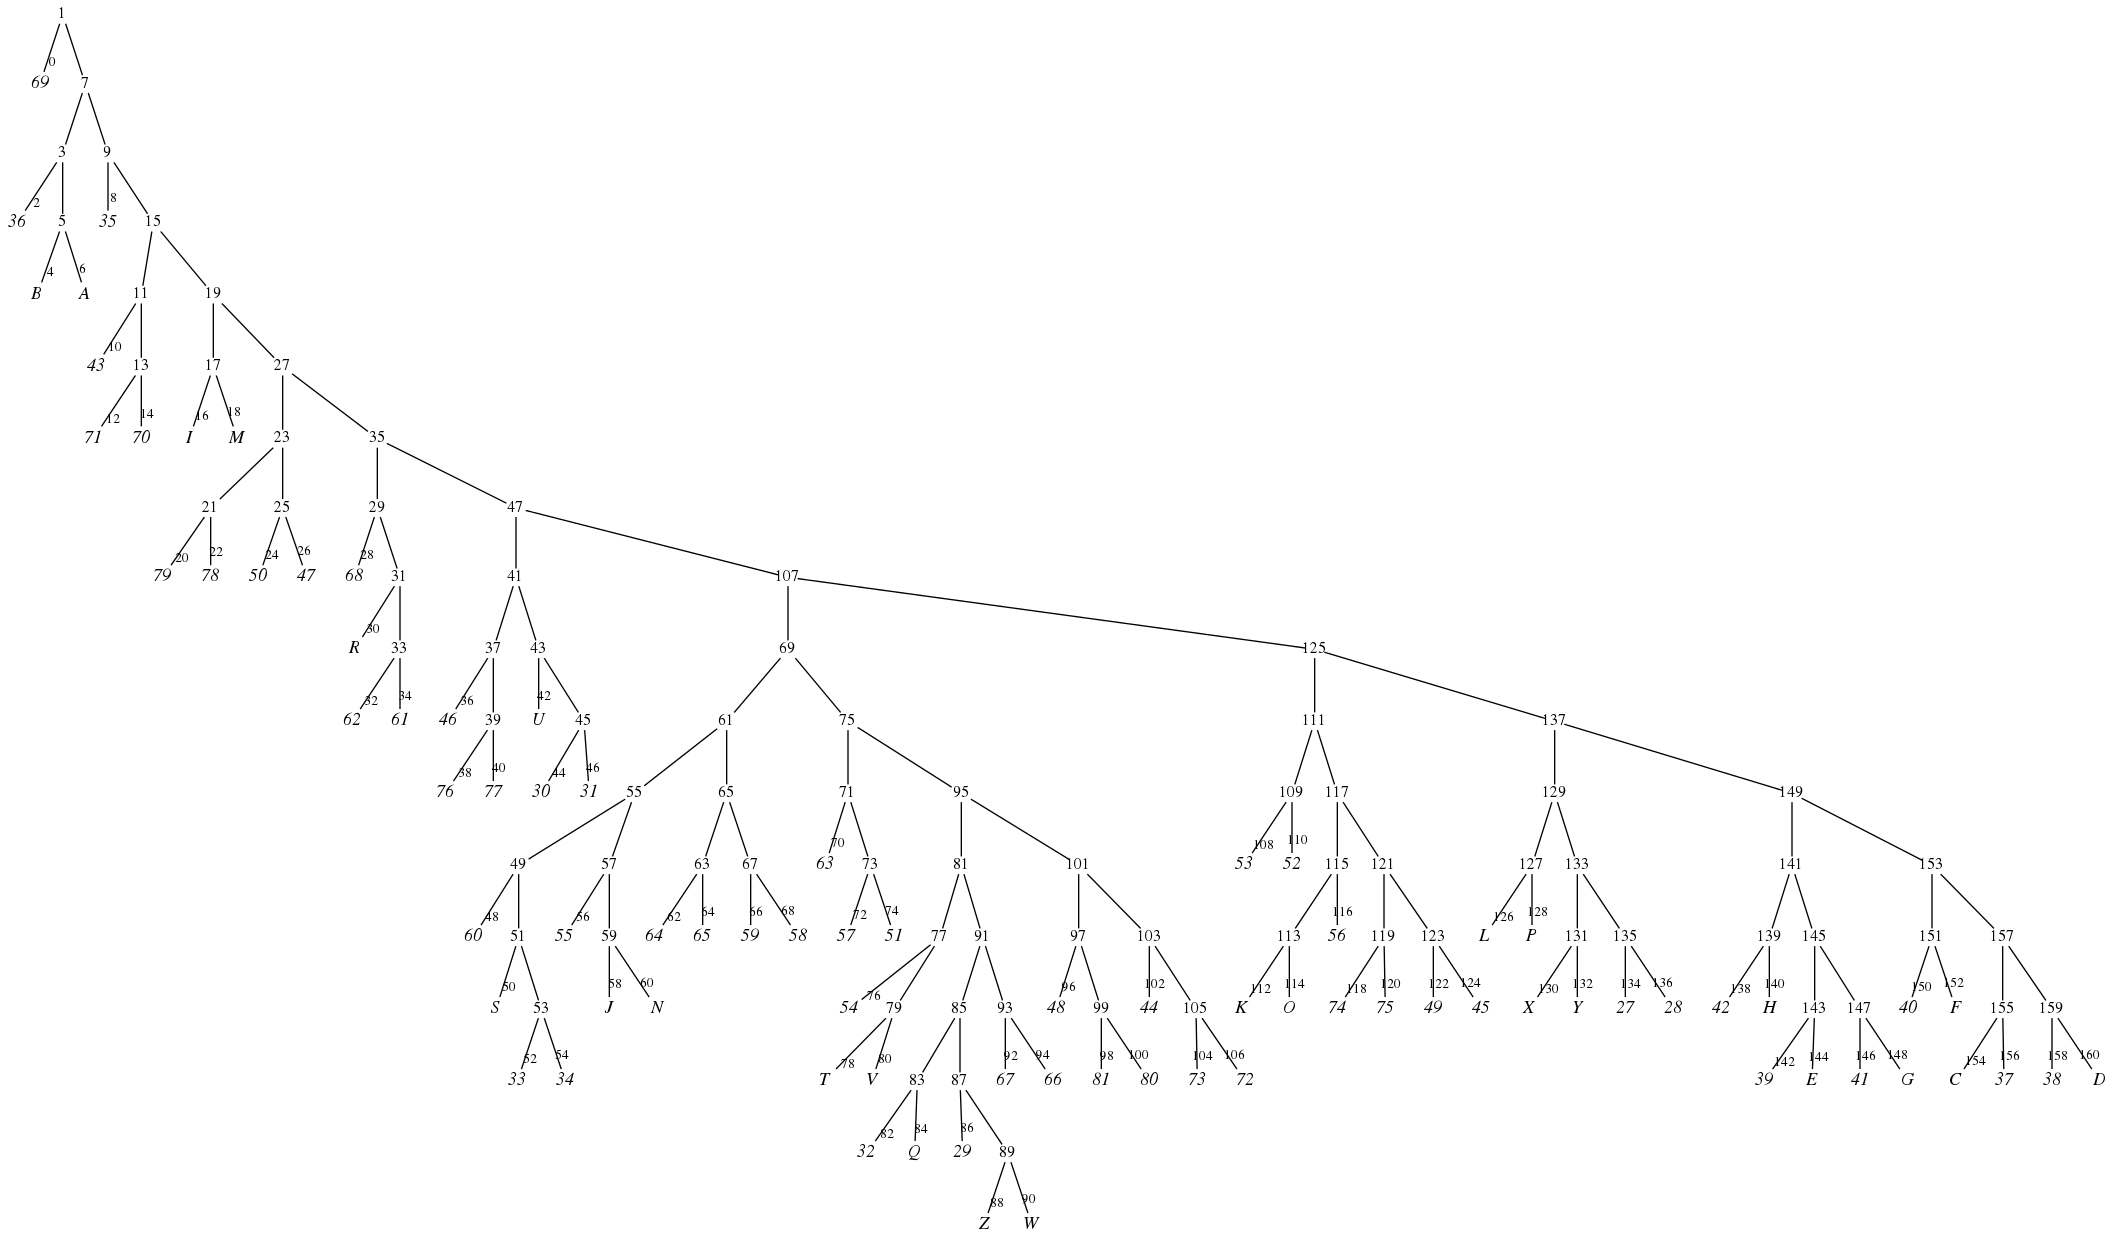
\includegraphics[scale=0.3]{largevtreeafterdao.png}
\caption{The manager's vtree at the end of a run of our model checker on crypto6, with an initial vtree of type balanced.}
\label{fig:large_vtree_after_reordering} 
\end{sidewaysfigure}
\begin{itemize}
\item The vtrees obtained after dynamic minimisation all seem to be \textit{very }similar in structure, whatever the initial vtree or the example considered. The vtree in Figure~\ref{fig:large_vtree_after_reordering} is a fair representative in terms of the size and structure of the l-subtrees.
\item The dynamic minimisation algorithm is ``symmetric" in the sense that it does \textit{not} force the vtree in one particular direction. It considers 24 vtrees (of which 12 are induced from the l-vtree by applying one of the usual vtree operations, and 12 arise from the r-vtree) and picks the best one. The fact that we get this vtree structure in all cases is evidence that it is in fact the \textit{ideal} configuration. 
\item One of the l-subtrees in the middle is very large -- it contains 30 variables, over a third of the total. This shows that smaller primes are \textit{not }necessary for an efficient computation, and that larger sets of variables may in fact improve it. 
\item It tends to happen (and it is definitely the case in Figure~\ref{fig:large_vtree_after_reordering}) that the first few l-subtrees are slightly smaller than the ones below. A reasonable explanation for this is that the first few l-subtrees correspond to the primes in the first few levels of the corresponding SDD (starting from the root), i.e those which need to be evaluated most often.
\end{itemize}
It is now even more evident that the l-subtree decomposition is a reasonable basis for vtree construction. We will take inspiration from these ``ideal" vtrees in order to find a more efficient alternative to the standard vtrees. 

\section{Static Comparisons with Alternative Vtrees}
\label{alternative}

In this section we explore and evaluate the various vtree constructions permitted by the l-subtree decomposition described in \ref{new_perspective}, and induced by the partition of the set of variables corresponding to the agents' variable allocation. We are still focusing on static vtree generation, so the dynamic minimisation features of both CUDD and the SDD Package are turned off.

This section is split into multiple subsections, each corresponding to a new investigation (but using the same construction process). At the beginning of each subsection, we describe the goal of the corresponding investigation and the particular vtree construction considered. We then present some experimental results and discuss any potential conclusions, which led us to the next investigation. 

Before we start, let us recall the setup: we are in the middle of verifying an interpreted system of agents, variable allocation \textit{has} taken place, and to each agent have been assigned three (distinct) sets of variables: state variables, primed state variables, and action variables. The union of the sets of each agent is the full set of variables used to encode the model. In order to construct a vtree for the model checker, we want to create a partition of this set which will be used to create the l-subtrees of the vtree. 

\subsection{A First Attempt Using Agent Variables}
\label{first_attempt}

The first vtree construction we consider is the most natural, and was already suggested as a starting point in \ref{vtree_options_in_practice}: we take the partition consisting of the variables allocated to each agent. That is, each agent corresponds to an l-subtree in the final vtree (strictly speaking, the last agent corresponds to the last \textit{few }l-subtrees of the vtree constructed). 

More specifically, for each agent we choose to construct a balanced subtree as according to the observations made in \ref{analysis_example}, it is the closest to the ideal vtree. We need to point out however, that constructing a perfectly balanced vtree for each agent is not often possible, as for this we would need the number of variables of each agent to be a power of 2.
We are particulatly interested in the following: \begin{enumerate}
\item The efficiency of this particular l-subtree decomposition;
\item The effect of changing the l-subtree order of the vtree;
\item The effect of changing the variable ordering induced by each l-subtree. 
\end{enumerate}
To evaluate these three parameters, we started our investigation with the most basic configuration: the l-subtrees were ordered using the \textit{agent order} (i.e. the way agent definitions are ordered in the ISPL file), and the variable ordering within each agent subtree was simply [state variables, primed state variables, action variables].

Then, we looked at the effect of changing the l-subtree order, by trying successively the \textit{inverse} of the agent order, and the \textit{ascending }order (in terms of the number of variables needed for each agent).

\begin{table}
\centering
\begin{tabular}{|*{8}{c|}}
\hline
& \multirow{2}{*}{BDDs} & \multicolumn{3}{c|}{$[s, s', a]$}& \multicolumn{3}{c|}{$[(s_1, s_1', ..., s_n, s_n'), a]$}\\ \cline{3-8}
& & Agent & Inverse & Ascending & Agent & Inverse &  Ascending \\ \hline
cryptos4 & 0.02 & 2.41 & 1.31 & 1.31& 0.24 & 0.15 & 0.15 \\ \hline
cryptos5 & 0.06 & 31.32 & 32.08 & 32.08&0.68& 0.31 & 0.31 \\ \hline
cryptos6 & 0.44 & 993.71& - & - & 4.05 & 1.01 & 1.01 \\ \hline
cryptos7 & 2.64 & - & - & - & 34.59 & 5.84 & 5.04\\ \hline
cryptos8 & 17.24 & - & - & - & - & 36.94 & 32.91 \\ \hline
cryptos9 & 98.95 & - & - & - & - & 271.16 & 248.18\\ \hline
pris6 & 0.15 & 7.43 & 3.94 & 2.52 & 2.02 & 2.16 & 1.03 \\ \hline
pris7 & 0.57 & 48.01 & 21.36 & 10.22& 8.31 & 8.63 & 3.61 \\ \hline
pris8 & 2.08 & 303.73 & 96.39 & 48.76 & 24.64 & 23.17 & 9.43 \\ \hline
pris9 & 11.47 &  & 3259.27 & 256.0 & 120.17& 109.24 & 38.75 \\ \hline
pris10 & 35.11 &  & - & - & 445.36& 347.23 & 128.1\\ \hline
nspk1 & 0.03 & 1.85 & 2.01 & 2.12 & 0.71 &0.81&  0.99\\ \hline
nspk2 & 2.71 & 542.32& - & - & 133.53 & 163.57 &  124.32\\ \hline
nspk4 & 0.32 & 68.95 &54.69 & 55.65 & 4.62 & 10.47 & 8.47\\ \hline
\end{tabular}
\caption{Vtree Option 5 -- Time}
\label{table:vtree5time}
\end{table}

\begin{table}
\centering
\begin{tabular}{|*{8}{c|}}
\hline
& \multirow{2}{*}{BDDs} & \multicolumn{3}{c|}{$[s, s', a]$}& \multicolumn{3}{c|}{$[(s_1, s_1', ..., s_n, s_n'), a]$}\\ \cline{3-8}
& & Agent & Inverse & Ascending & Agent & Inverse & Ascending\\ \hline
cryptos4 & 11 & 59 & 44 & 44 & 6 & 3 &  \textbf{3}\\ \hline
cryptos5 & 18 & 673 & 574 & 574 &31 & 7 &  \textbf{7}\\ \hline
cryptos6 & 45 & 8716 & 
- & - & 196& 33 &  \textbf{33} \\ \hline
cryptos7 & 160 & - & - & - & 1367 & 170 & 165 \\ \hline
cryptos8 & 647 & - & - & - & - & 997 & 974\\ \hline
cryptos9 & 2850 & - & - & - & - & 5270 & 5066 \\ \hline
pris6 & 31 & 76 & 45 & 52 & 42&31&  \textbf{29}\\ \hline
pris7 & 48 & 316 & 141 & 158 & 127 &88 & 83\\ \hline
pris8 & 102 & 1558 & 483 & 744& 387 & 116 & 233\\ \hline
pris9 & 313 &  &9000  & 3052 & 1418 & 700 & 724\\ \hline
pris10 & 847 &  & - & - & 5255 & 2059 & 2435\\ \hline
nspk1 & 16 & 27 & 29 & 25  & 11 & 13 &\textbf{13} \\ \hline
nspk2 & 324 & 2949 & - & - & 1301 & 1374 & 1396 \\ \hline
nspk4 & 92 & 685 & 884 & 901& 63&81&  \textbf{85}\\ \hline
\end{tabular}
\caption{Vtree Option 5 -- Memory}
\label{table:vtree5memory}
\end{table}


Finally, we evaluated the impact of the variable order of each balanced subtree, and tried various orderings, in particular the equivalent of the MCMAS standard ordering 2, namely $$[\mbox{(states and primed states interleaved)}, \mbox{actions}].$$

Tables~\ref{table:vtree5time} and \ref{table:vtree5memory} contain our experimental results. It appears very clearly that the second variable ordering (MCMAS number 2) is \textit{much }more efficient than the original one, in all cases. This is somewhat surprising, since when we compared balanced subtrees in \ref{balanced_comparisons}, we concluded that the impact of the variable ordering differed a lot depending on the model. Yet, when these balanced subtrees are used as l-subtrees of a larger vtree, the results are more constistent, and there is a clear winner.

Concerning the impact of the l-subtree order in the vtree, the conclusion is less obvious from the tables alone, and again, it seems to depend on the model. We inspect the results a little more closely. In a majority of cases, it appears that leaving the bigger agent subtrees at the bottom of the vtree (using the ascending order) reduces computation times. But this is not always the case.

For the dining cryptographers in particular, when the SDD sizes exceed a certain number, it is more efficient to leave the Environment subtree (the bigger one by far, and the first in the agent order) at the top of the vtree. One possible explanation is that in this model, the transition relation for the Environment is \textit{considerably} larger than that of individual Cryptographers, therefore the major part of the computation time is spent in the reachable state-space computation, applying this particular relation (the others are negligible). The time gained by facilitating this unique operation therefore makes a more significant difference than that of facilitating all the others. 

We suspect that for the NSPK examples, where results are also a little inconsistent, the same problem occurs. However, this is harder to analyse, considering agents in these examples have comparable numbers of variables. 

It is also interesting to compare the time and memory usage in different runs of the same example, but with different vtrees. A few ``irregularities" can be found there too, which confirms the fact that the size of the data structures is not the only thing affected by the vtree, but the efficiency of operations is too. 
This was much less appearant in the case of right-linear vtrees (i.e. changing the variable ordering of a right-linear vtree keeps the ratio constant, whereas changing the structure of the vtree makes it vary). 

We can conclude that when l-subtrees correspond to agent variable sets,\begin{itemize}
\item The most efficient variable order with this is the equivalent of the standard order number 2 in MCMAS;
\item Ordering the subtrees with respect to their size is unpredictable.
\end{itemize}
To prevent this uncertainty, we had the idea of setting an \textit{upper bound} on the size of the l-subtrees in the vtree that we construct. This is the next investigation.

\subsection{An Upper Bound on the Size of Subtrees}

Theoretically, setting a maximum number of variables per l-subtree should prevent the lengthy operations sometimes caused by an irregularity in the number of variables allocated to various agents, as described above. Whether or not this will reduce the \textit{total} computation time, or the size of the resulting SDDs, is still to determine. 

In this subsection, we start with the same partition of the set of variable as in the previous one (i.e. the partition arising from agents), however we \textit{bound }the size of each set in the partition by a given integer $N$. This means that if an agent has been allocated more than $N$ variables, it will be ``represented" by two or more l-subtrees in the final vtree.
With these experiments, we try to explore the following questions:\begin{enumerate}
\item What is an appropriate upper bound $N$? Should it depend on the total number of variables?
\item When l-subtrees are limited to a size of $N$ variables, does their order still matter?
\item If we need to split an agent's variable set into multiple subsets, how should we arrange the variables? 
\item Does any of the above lead to an improvement on the vtree defined in the previous subsection?
\end{enumerate}
To investigate these questions, and draw conclusions as accurately as possible, we make some experiments.

We start by comparing different values of the upper bound $N$, which we define as a function of the total number of variables, denoted $n$. The main reason for using a function rather than a constant is that for larger-scale models, where agents have a large number of variables, a small upper bound is likely to slow down the process rather than accelerate it -- we do not want to lose the value that l-subtrees are here to add in the first place (that is, to lower the number of \textit{decisions} to make). That said, we choose functions which "grow slowly", so that even for \textit{very }large-scale models, the upper bound is still reasonably low. 

As shown in Tables~\ref{table:upperboundvaluestime} and \ref{table:upperboundvaluesmemory}, we used three different functions for this experiment: $N = log_2(n), N = \sqrt{n}$ and  $N = 2log_2(n)$, where for each example, we round up $N$ to the nearest integer. These functions almost behave like constants on the set of examples that we look at. As an indication, we give the actual values of $N$ for each example, in each case, in the table below: \\

\begin{table}
\centering
\begin{tabular}{|*{5}{c|}}
\hline
& \multirow{2}{*}{BDDs} & \multicolumn{3}{c|}{Values of $N$}  \\ \cline{3-5}
&  & $log_2(n)$ & $\sqrt{n}$ & $2log_2(n)$  \\ \hline
cryptos7 & 2.64 &1.51 & 1.21 & 1.02 \\ \hline
cryptos8 & 17.24 & 5.70 & 4.78 & 4.90 \\ \hline
cryptos9 & 98.95 & 30.46& 27.51  & 63.06 \\ \hline
pris9 & 11.47 & 42.17 & 32.86 & 27.98  \\ \hline
pris10 & 35.11 & 157.01 & 112.781  & 102.0 \\ \hline
nspk1 & 0.03 & 0.55 & 0.48& 0.65 \\ \hline
nspk2 & 2.71 & 27.88 &20.15 & 20.05 \\ \hline
nspk4 & 0.32 & 3.94 & 5.12 & 4.16 \\ \hline
nspk5 & 158.62 & -& 859.42& 782.07 \\ \hline
\end{tabular}
\caption{Time Comparisons With Different Values of the Upper Bound $N$. In the table, $n$ denotes the total number of variables in the model.}
\label{table:upperboundvaluestime}
\vspace{1in}
\centering
\begin{tabular}{|*{5}{c|}}
\hline
 & \multirow{2}{*}{BDDs} & \multicolumn{3}{c|}{Values of $N$}  \\ \cline{3-5}
 & & $log_2(n)$ & $\sqrt{n}$ & $2log_2(n)$  \\ \hline
cryptos7 & 160 & 65 & 56  & 51 \\ \hline
cryptos8 & 647 & 216 & 188 & 154 \\ \hline
cryptos9 &2850& 1117 & 886  & 1350\\ \hline
pris9 & 313 &1086 & 718  & 698\\ \hline
pris10 & 847& 3464 & 2576 & 2262\\ \hline
nspk1 & 13 & 12 & 12  &  12\\ \hline
nspk2 & 135 & 370 & 273  & 257\\ \hline
nspk4 & 45 & 89&78  & 72 \\ \hline
nspk5 & 3841 & - & 6378 & 5876  \\ \hline
\end{tabular}
\caption{Memory: Different Values of the Upper Bound $N$. }
\label{table:upperboundvaluesmemory}
\end{table}

{\centering
\begin{tabular}{*{3}{c|}c}
Example & $log_2(n)$ & $\sqrt{n}$ & $2log_2(n)$  \\
\hline
cryptos7 & 7 & 10 & 14   \\
cryptos8 & 7 & 11& 14 \\
cryptos9 & 7& 11 & 14  \\
pris9 & 7& 9 & 13   \\
pris10 & 7& 10 & 13   \\
nspk1 & 7& 9 & 13   \\
nspk2 & 7& 11 & 14  \\
nspk4 & 7& 11 & 14   \\
nspk5 & 8& 14 & 15   \\
\end{tabular}
\\\vspace{0.5in}}

\noindent It is clear from the results that setting an upper bound \textit{does} reduce SDD computation times significantly, to the point where the SDD computations are around \textit{three times faster} than the BDD computations in the case of the dining cryptographers, and at a comparable level (the difference being less than an order of magnitude) in all other cases. Observe that this is the first time we have achieved faster computations than with right-linear vtrees. It is also the first time we have managed to verify NSPK, version 5 with SDDs without running out of memory.

On the other hand, the upper bound itself doesn't seem to have such a big impact on the computation: none of the ones we tried seems to come out as a more efficient solution than the others in the general case. Our conclusion from this is that it is sufficient to ``smoothen" the vtree by splitting up the very large l-subtrees, but it does not matter too much how small the resulting l-subtrees are. 

These results confirm our hypothesis that large l-subtrees are ``blocking" the computation at various steps of the execution, and that they were the main factor of the slow performances obtained in our previous experiments, particularly with the left-linear and vertical vtrees.
\\\\
Recall now that in \ref{first_attempt} we experimented with different \textit{orderings }of the vtree's l-subtrees. We saw that these had a relatively important effect on the efficiency of the computation, and we concluded that the \textit{irregularity} in the number of variables allocated to each agent was the main cause of this effect, as changing the order would mean shifting very large l-subtrees up and down the vtree (leading to an important change in the SDDs themselves). 

Now that we have an upper bound on the l-subtree size, we would like to find out whether changing this ordering still has such a big impact. More generally, we would like to know the impact of the way we re-arrange variables when splitting an l-subtree due to its size exceeding the upper bound $N$. In the following experiment, we set the upper bound to be $N = \sqrt{n},$ and we compare the following three vtree constructions: 
\begin{enumerate}
\item The l-subtrees are still balanced and in the agent order, and if one of them has size $> N$, we split it into two (or more) l-subtree and put the second one (and the ones after, if any) immediately after in the final vtree.
\item The l-subtrees are still constructed and split in the same way, but in the final vtree we order them in ascending order of size. 
\item Instead of starting with one l-subtree per agent, we start with two: one containing state and primed state variables, and another containing action variables. We then split any of them whose size exceeds $N$, and leave them in the same order as agents to construct the vtree. 
\end{enumerate}
The first of these three constructions is essentially the one used in the last experiment, which we include here for comparison purposes. The second one will help us explore whether the l-subtree order matters, and the third will tell us whether re-arranging the variables in a more meaningful way \textit{might} lead to an improvement of the computation time (more meaningful, because a split is less likely to occur at a random place in the variable list, considering we force it to happen between action and state variables).

\begin{table}
\centering
\begin{tabular}{|*{5}{c|}}
\hline
& \multirow{2}{*}{BDDs} & \multicolumn{3}{c|}{Vtree Construction} \\ \cline{3-5}
& & 1. & 2. & 3.\\ \hline
cryptos7 & 2.64 &  1.21& 1.33 & 2.26 \\\hline
cryptos8 & 17.24&  4.78& 4.09 & 8.36 \\\hline
cryptos9 & 98.95 &27.51 & 20.343 & 42.60 \\\hline
pris9 & 11.47&32.86 & 41.14 & 86.98\\\hline
pris10 & 35.11&112.78& 105.16 & -\\\hline
nspk1 & 0.03 &0.48  & 0.46 & 0.31 \\\hline
nspk2 & 2.71 &  20.15& 36.675 & 20.63 \\\hline
nspk4 & 0.32 & 5.12& 4.94 & 3.11 \\\hline
nspk5 & 158.62 &859.2 & - & 1062.52\\\hline
\end{tabular}
\caption{Time}
\label{table:vtree6time}
\vspace{1in}
\begin{tabular}{|*{5}{c|}}
\hline
& \multirow{2}{*}{BDDs} & \multicolumn{3}{c|}{Vtree Construction} \\  \cline{3-5}
& & 1. & 2. & 3.\\ \hline
cryptos7 & 160 & 56 & 47 & 95 \\\hline
cryptos8 & 647 & 188 & 175& 350 \\\hline
cryptos9 & 2850 & 886 & 732 & 1751 \\\hline
pris9 & 313 & 1086 & 844& 2796 \\\hline
pris10 & 847 & 3464 & 1919 & - \\\hline
nspk1 & 13 & 12& 13 & 9 \\\hline
nspk2 & 135 & 370 & 482 & 291 \\\hline
nspk4 & 45 & 78  & 120 & 69 \\\hline
nspk5 & 3841 & 6378 & - & 7849 \\\hline
\end{tabular}
\caption{Memory}
\label{table:vtree6memory}
\end{table}

The results are in Tables~\ref{table:vtree6time} and \ref{table:vtree6memory}. We can see that none of the new configurations (2. and 3. in the tables) are particularly striking improvements on the one we had before (1. in the table). 

Perhaps surprisingly, the ``more meaningful" third construction actually seems to make things worse in a majority of cases. We also tried (although without showing the results here) similar constructions where all action l-subtrees are kept at the top, or the bottom of the vtree, rather than next to their corresponding state l-subtrees, as in 3. These were even more inefficient (on our set of models).
 The conclusion we draw from this is that when considering the bounded vtree construction presented in this section, any reordering set to occur \textit{after} splitting is not particularly efficient; although it may not necessarily lead to worse computation times, in all the cases we tried it never improved them. This could perhaps be explained by the fact that action variables are only used in the SDDs for transition relations, which also use state and primed state variables; not separating them completely might therefore be a better idea.
 \\\\
Overall, it seems that setting an upper bound on the l-subtree size does lead to a much more efficient performance, and this was very clear in all of our experiments. However, reordering l-subtrees after splitting doesn't seem to give particularly interesting results, and is probably not worth it, as it presents a risk of separating variables which would have been more efficient closer together. 

Before moving on, we want to insist on the fact that the use of \textit{balanced} l-subtrees seems essential to the efficiency of this vtree construction. Early on in the project, we experimented with right-linear, and left-linear vtrees as l-subtrees; the results were \textit{not} satisfying, and we chose not to include them in this report, in order to keep the focus on the balanced approach.

\subsection{A Different Partition of the Set of Variables}

The objective of this subsection is to explore different \textit{partitions} of the set of variables as bases for the l-subtree construction, diverging from the purely ``agent-based" approach taken so far. 

Before we propose a replacement partition, we want to make the assumption that we are better off keeping the action variables of an agent close to each other in the vtree, preferably contiguous. This is based on the fact that it is often the case for vtrees produced by the dynamic minimisation algorithm, even though these were completely re-structured; it is for instance true with most agents in
 Figure~\ref{fig:large_vtree_after_reordering}.
(Of course, it may well be possible to generate good vtrees without respecting this assumption. It seems however that this is one principle that the dynamic search agrees with, that we can easily follow, and with which we have obtained good results so far).

So, what are our options? Recall that we still need to find a way of generating the vtree which ``makes sense", i.e. which is dependent on the abstract structure of a multi-agent system, rather than on a specific model or example. 
We propose the following vtree construction:
\begin{itemize}
\item We create balanced l-subtrees which contain 2 variables from each agent, a state variable and its primed counterpart;
\item We continue until all agents have run out of variables (i.e l-subtrees get smaller as the process goes on);
\item For action variables, we give ourselves two options: we can create an l-subtree containing \textit{all }the action variables (option 1), or we can create one action l-subtree for each agent (option 2). 
\end{itemize}

TODO changer le troisieme point au desssus et analyse + conclusion

The results are in Table~\ref{table:newpartition}.
\begin{table}
\centering
\begin{tabular}{|*{5}{c|}}
\hline
 & \multicolumn{2}{c|}{BDDs} & \multicolumn{2}{c|}{SDDs - New Partition } \\ \cline{2-5}
 & Time & Memory & Time & Memory \\ \hline
cryptos7 &2.64& 160& 1.41 & 75 \\ \hline
cryptos8 &17.24& 647& 5.05 & 264 \\ \hline
cryptos9 &98.95 &2825& 20.36 & 969 \\ \hline
pris9 &11.47 &313& 59.88 & 1516 \\ \hline
pris10 &35.11& 847& 197.95 & 4341 \\ \hline
nspk1 &0.03& 13 & 0.57 & 17 \\ \hline
nspk2 &2.71& 135& 83.62 & 932 \\ \hline
nspk4 &0.32& 45 & 11.09 & 219 \\ \hline
nspk5 &158.62& 3841& - &-  \\ \hline
\end{tabular}
\caption{Time and Memory: new partition}
\label{table:newpartition}
\end{table}


\section{Dynamic Variable Reordering and Minimisation}

Dynamic minimisation is very important. In the case of BDDs, it consists in reordering the variables; for SDDs it is about searching for a better vtree -- all of this \textit{while} the program is running. Turning on the dynamic variable reordering feature in MCMAS allows for \textit{much larger} models to be verified.

In this section, our objectives are the following:
\begin{enumerate}
\item Evaluate the efficiency of the dynamic minimisation feature in the  SDD Package, exploring various \textit{initial} vtrees, identifying some of the better ones in the context of model checking; 
\item Compare the performance of our own implementation of a dynamic minimisation algorithm (see \ref{dynamic_with_sdds_implementation}) against the one included in the SDD Package;
\item Ultimately, compare the performance of our model checker with that of MCMAS when both dynamic minimisation features are enabled.
\end{enumerate}
In addition, we will explore another aspect of dynamic minimisation, namely the \textit{configuration} of the SDD manager, including the thresholds, time and memory limits to be applied in the dynamic vtree search algorithm. 

\subsection{The Default Dynamic Minimisation Function}

In this first subsection, we experiment with the dynamic minimisation feature using its default behaviour, while changing the \textit{initial }vtrees (i.e. the vtree the manager was constructed with). Tables \ref{table:defaultdaotime} and \ref{table:defaultdaomemory} contain the results obtained with seven different initial options: \begin{itemize}
\item Options 1 to 4: the four standard vtrees, in the order used previously, namely right-linear, balanced, left-linear, vertical. All of these vtrees were constructed with standard ordering 2.
\item Option 5: a single balanced l-subtree for each agent (as in \ref{first_attempt}), in ascending order of size
\item Option 6: the ``bounded version" of option 5 (as in \ref{upper_bound})
\item Option 7: a single \textit{right-linear} vtree for each agent (non-bounded). This has not been tried before.
\end{itemize}
Our first observation is the very low memory usage of the model checker in this situation. As previously mentioned, the dynamic minimisation feature triggers the garbage collector, which explains those results. As opposed to all the previous experiments, the memory usage and execution time of the program are now completely unrelated, and one can no longer be ``guessed" from the other. From now on, considering the vast majority of our memory results are very acceptable, we will mostly be commenting on the computation times.

Our second observation is that no initial vtree stands out. By this, we certainly do not mean that all of them lead to the same computation time, but rather that it seems to vary a lot depending on the example. Furthermore, we notice a very important irregularity even within the same example class. For the dining cryptographers, an initial right-linear vtree (option 1) seems to make the $n=12$ version \textit{slower }than the $n=15$, which is not what is expected. 

These inconsistencies are interesting, because they demonstrate, once again, the impact of the vtree and the difficulty in finding a good one. The search algorithm must have been ``luckier" in the case $n=15$ than it was for $n=12$, or perhaps the ``ideal" vtree was ``closer" to a right-linear vtree in the first case, so the algorithm got to it faster. (Pardon the extensive use of quotation marks, but omitting them would imply the existence of a such notions, which are probably very subjective.)

This does however raise the question of the \textit{distance} between two vtrees, which seems fundamental in the search for an initial vtree for this particular algorithm which navigates the whole space of vtrees. We will not investigate this further in this project, although it seems that it would be an interesting perspective, and that the \textit{geometry} of the space of vtrees would surely give us useful information on how to navigate it more efficiently. 

The final comment we make is that although no vtrees stand out as the best, left-linear vtrees are clearly some of the worst and should probably not be used as initial vtrees. One possible explanation for this is that the number of vtree operations required to obtain an acceptable vtree (similar to the one in Figure~\ref{fig:large_vtree_after_reordering}, which is what the algorithm seems to be reaching for) is higher than for other vtrees. 

These results are \textit{slower} than those obtained with MCMAS, for all examples. From now on, we only compare different vtrees to each other. We discuss the comparison between both model checkers in \ref{daocomparison}. 

\begin{table}
\centering
\begin{tabular}{|*{8}{c|}}
\hline
& 1 & 2 & 3 & 4 & 5 & 6 & 7 \\ \hline
cryptos9 & 6.62 & 4.60 & 12.41 & 12.96 & 2.42 & 1.74 & 3.17\\ \hline
cryptos12  & 52.74 & 3.22 & 26.2 & 65.18 & 6.63  & 15.21 & 15.54 \\ \hline
cryptos15   & 19.93 & 66.07 & 257.09 & - & 12.58 & 21.15 & 22.35 \\ \hline
pris10 & 22.4 & 77.33 & 465.14 & 48.35 & 90.8 & 107.9 & 32.91 \\ \hline
pris11 & 218.45 & 115.85 & 283.67 & 186.15 & 103.97 &268.32  & 157.3 \\ \hline
pris12 & 219.98 & 585.11 & 983.0 & 162.6 & 344.76 & 290.53 & 151.26 \\ \hline
nspk2 & 266.8 & 50.23 & 181.95 & 39.08 &105.57 & 181.31 & 117.79 \\ \hline
nspk4 & 30.31 & 55.85 &75.43& 72.51 & 39.7 & 70.08 & 34.56\\ \hline 
nspk5 & - &-  &- & - &- & - & -\\ \hline
\end{tabular}
\caption{Time}
\label{table:defaultdaotime}
\vspace{0.5in}
\centering
\begin{tabular}{|*{8}{c|}}
\hline
& 1 & 2 & 3 & 4 & 5 & 6 & 7 \\ \hline
cryptos9 & 10& 12 & 26 &22  & 4 & 4 & 4\\ \hline
cryptos12 & 87 & 3 & 38 & 36 & 6 &12 & 8 \\ \hline
cryptos15 & 32 & 1175 & 735 & - & 15& 14 & 15\\ \hline
pris10 &8 & 17 &23 & 15 & 12 & 44 & 10\\ \hline
pris11 & 34 & 619 & 64 & 25 & 106 & 70 & 15\\ \hline
pris12 & 31 & 45 & 89 & 40 & 46 & 30 & 23\\ \hline
nspk2 & 289 &62 & 114 & 62 & 60 &94 & 65\\ \hline
nspk4 &31  & 36  &39 & 72 & 18 & 32& 50 \\ \hline
nspk5 &  - & - & -& - & -& - & -\\ \hline
\end{tabular}
\caption{memory}
\label{table:defaultdaomemory}
\end{table}

\subsection{Changing the Configuration}

In this section, we attempt to reduce computation times by exploring alternative \textit{configurations} of the SDD manager. Mainly, this involves modifying thresholds, time and memory limits for vtree operations and minimisation.

Recall that at each step of the dynamic vtree search, the manager attempts to compute 24 alternative vtrees (see \ref{sdd_dao_algo} for details), and selects the best one. Out of those 24 vtrees, some might lead to a important increase in the size of the SDD nodes, and checking this might potentially take a long time. For this reason, the SDD Package sets limits on the size increase and time of each vtree operation, to prevent the overhead from being too significant. These size and time limits can be modified by the users, and they will be the focus of our investigation. 

Before we start, we inspect the SDD ``statistics" provided by the manager at the end of the execution of the program, which indicate the number of vtree operations which have been prevented by the manager. In the vast majority of cases, no operations have been rejected due to them being over the time limit. However, a large number of them (often over $10^5$, even for small examples) seem to be turned down because of an important size increase. It therefore seems more important that we explore this aspect of the configuration.

The size limit is supplied as an ``increase percentage", so a size limit of 1.1 will prevent the size of an SDD node from growing more than 10\%. This is the default option, and in our experiments we compare this with runs of the model checker with limits of 1.01 and 1.4. These results are presented in Tables~\ref{table:newconftime} and \ref{table:newconfmemory}. 

The default option is clearly the best one out of those three. It seems that the lower limit prevents so many vtree operations from happening, that the algorithm fails to find an efficient enough vtree. In particular, memory results are very high compared to what we usually obtain when the garbage collector enough. On the other hand, a higher limit seems to waste a lot of time applying numerous vtree operations which, looking at the results, are not worth the time spent. 

\begin{table}
\centering
\begin{tabular}{|*{4}{c|}}
\hline
 &1.01 & 1.1 & 1.4 \\ \hline
cryptos9 & 8.30 & 2.42 & 3.70 \\ \hline
cryptos12  & 25.43 & 6.63 & 11.55 \\ \hline
cryptos15 & 114.169 & 12.58 & 19.45 \\ \hline
pris10 & 211.11 & 90.8 &165.84  \\ \hline
pris11 & 335.65 & 103.97 & 510.32 \\ \hline
pris12 & 268.24 & 344.76 & 613.84\\ \hline
nspk2 & 99.17 & 105.57 & 159.77 \\ \hline
nspk4 & 17.34 & 39.7 & 187.65 \\ \hline
nspk5 & - & -&  -\\ \hline
\end{tabular}
\caption{Time}
\label{table:newconftime}
\vspace{1in}
\centering
\begin{tabular}{|*{4}{c|}}
\hline
 &1.01 & 1.1 & 1.4 \\ \hline
cryptos9 & 68 & 4 & 3 \\ \hline
cryptos12 & 68 &6 & 15 \\ \hline
cryptos15 & 399 &15& 9 \\ \hline
pris10 & 710 & 12 & 26 \\ \hline
pris11 & 252 & 106  &  29 \\ \hline
pris12 & 132 &46 & 25 \\ \hline
nspk2 & 122 & 60 & 50 \\ \hline
nspk4 & 57 & 18 & 49\\ \hline
nspk5 & - & - & -\\ \hline
\end{tabular}
\caption{memory}
\label{table:newconfmemory}
\end{table}



\subsection{The New Dynamic Minimisation Function}


\begin{table}
\centering
\begin{tabular}{|*{4}{c|}}
\hline
 &5 & 6 & 7 \\ \hline
cryptos9 && &\\ \hline
cryptos12  &&  & \\ \hline
cryptos15   &&  & \\ \hline
pris10 &  && \\ \hline
pris11 & & & \\ \hline
pris12 & && \\ \hline
nspk2 & & & \\ \hline
nspk4 & && \\ \hline
nspk5 &&& \\ \hline
\end{tabular}
\caption{Time}
\label{table:newdaotime}
\vspace{1in}
\centering
\begin{tabular}{|*{4}{c|}}
\hline
& 5 & 6 & 7\\ \hline
cryptos9 & & & \\ \hline
cryptos12  &  && \\ \hline
cryptos15   &  && \\ \hline
pris10 &&  & \\ \hline
pris11 & & & \\ \hline
pris12 & && \\ \hline
nspk2 &  && \\ \hline
nspk4 & && \\ \hline
nspk5 &  && \\ \hline
\end{tabular}
\caption{memory}
\label{table:newdaomemory}
\end{table}

\subsection{Comparison with the MCMAS dynamic minimisation feature} 
\label{daocomparison}

In this final subsection, we compare the results obtained for SDD dynamic minimisation in our model checker with the BDD variable reordering functionality implemented in MCMAS. Table~\ref{table:dynamiccomparisonwithmcmas} contains both the time and memory results of our comparison. The BDD results were obtained by running MCMAS using the standard ordering 2 as the initial variable order. The SDD results do not correspond to one experiment in particular, but instead were taken as the \textit{shortest} of all the computation results obtained previously. Memory and time results do however correspond to the same run of the model checker.

Although this is not really a fair comparison, it is enough for us to realise that BDDs \textit{massively} outperform SDDs, when both minimisation features are activated. This could have been expected, as there are two major reasons for this: \begin{enumerate}
\item Vtree search is a much more time-consuming process, as seen earlier in this report. It is very likely that the structures obtained after a good vtree search are more compact than the corresponding BDDs, however the difference in size does not make up for the time required for the search -- at least in our examples.
\item In CUDD are implemented 14 different variable reordering techniques \cite{CUDD_website}. Some of these were designed specifically for the development of the library, and the rest were taken from the large amount of existing research on BDD minimisation. In comparison, only one SDD minimisation algorithm has been proposed, and it was not designed for model checking but for knowledge compilation, which requires far less operations on SDDs. 
\end{enumerate}



\begin{table}
\centering
\begin{tabular}{|*{5}{c|}}
\hline
 & \multicolumn{2}{c|}{Time} & \multicolumn{2}{c|}{Memory} \\ \cline{2-5}
 & BDDs & SDDs (min.) & BDDs & SDDs (min.) \\ \hline
cryptos9 & 0.33 & 1.74 & 12 & 4 \\ \hline
cryptos12 & 0.90 & 3.22  & 13 & 3 \\ \hline
cryptos15 & 7.19 & 12.58 & 32 & 15 \\ \hline
pris10 & 0.61 & 22.4 & 32 & 8\\ \hline
pris11 & 0.94 & 103.97 & 44 & 106 \\ \hline
pris12 & 1.61 & 151.26 & 47 & 23 \\ \hline
nspk2 & 12.53 & 39.08 & 43 & 62 \\ \hline
nspk4 & 5.68 & 17.34 & 20 & 57 \\ \hline
nspk5 & - & - & -& - \\ \hline
\end{tabular}

\caption{Dynamic Comparison with MCMAS: Time and Memory}
\label{table:dynamiccomparisonwithmcmas}
\end{table}

\section{Existential Quantification}

In these final experiments, we evaluate our new implementation of the existential quantification of a set of variables, as detailed in \ref{exist_implementation}. Recall that the default \texttt{exists} algorithm in CUDD is recursive, whereas no such implementation exists in the SDD Package, leaving us with the basic method of iterating over the set of variable, which seems like a slower method. For this reason, we implemented the equivalent of CUDD's recursive algorithm in our model checker, hoping to reduce execution times. 

Table~\ref{table:existcomparisons} contains the results of our comparisons of both algorithms, with BDDs, and SDDs with both right-linear and ``bounded agent-based" vtrees. 

In the case of BDDs, the recursive algorithm performs slightly better, as we expected. However, the SDD results are rather suprising at first sight, considering the iterative algorithm is more efficient in most cases. 
We need to point out one thing before we give our analysis of the situation: the dashes `-' in that tables are due to a problem in the recurse


\begin{table}
\centering
\begin{tabular}{|*{7}{c|}}
\hline
 &\multicolumn{2}{c|}{\multirow{2}{*}{BDDs}} & \multicolumn{4}{c|}{SDDs}  \\ \cline{4-7}
 & \multicolumn{2}{c|}{}& \multicolumn{2}{c|}{right-linear}& \multicolumn{2}{c|}{bounded agents}\\ \hline
 & recurs. & iter. & recurs. & iter. & recurs. & iter. \\ \hline 
cryptos8 &17.24 & 18.53 & 30.51 & 30.42 & 10.49 & 5.70\\ \hline
cryptos9 & 98.95  & 109.29 & 149.08 & 145.313 & 53.59 & 30.46\\ \hline
pris8 & 2.03 & 4.05  & 69.73&64.43  &43.67 & 29.696 \\ \hline
pris9 & 11.47& 18.42 & - & 252.21 & -& 42.17 \\ \hline
nspk2 & 2.71 & 8.97 & - & 76.32 & -& 27.88\\ \hline
nspk4 & 0.32 & 0.91 & - & 9.79 & 29.28 & 3.94 \\ \hline
\end{tabular}
\caption{Comparisons of various exists functions}
\label{table:existcomparisons}
\end{table}

\section{Summary}

STATIC 
- standard not efficient
- by agent, better but not so good
- bound it to get rid of irregularities, it works well. summarize (1) the order and (2) the bound
- try a new partition but didn't find anything as efficient, this is logical because it's not as natural

DYNAMIC 
- hard to find heuristics because it varies so much
- 1.1 size is the best
- New grouped implementation does not work well, if we had more time we w
-

\section{Qualitative Evaluation}

\subsection{Evaluation of the evaluation}

-Our research is a good basis, and we evaluated a lot of different things
-perhaps not in too much depth
-also to explain the results better it would have been useful to have access to the SDD package code 
- should have done more research on memory management..packages rely a lot on the cache

\subsection{Evaluation of the Code}

not a great design, and code is messy

\subsection{Project Limitations}

THINGS WE DIDN'T DO BUT SHOULD HAVE DONE: 
- the debugging thing
- go into more depth in evaluation

\chapter{Conclusion and future work}

ARE BDDs REALLY BETTER?
yes but SDDs still impressive (that they sometimes beat BDDs even though manager is much worse)


REVIEW
- very interesting project because of its potential
- basis for further improvement on SDDs, it is possible!
- project is useful for any other use of SDD, perhaps knowledge compilation (although agent-based approaches won't work)

FUTURE WORK: 
- ADDs
- new grouped implementation, being able to specify actual groups
- Studying geometry of the space of vtres
- 


\section{Review}

\section{Future work}

Missing features will be counterexample/witness generation, and checking for deadlock or model overflow. Also being able to check ATL formulas.
At some point I would like to have a go at implementing an ADD equivalent for SDDs.
-> Call \texttt{sdd\_apply()} on a reduced vtree


\begin{thebibliography}{9}

\bibitem{original_model_checking} E. M. Clarke, E. A. Emerson: \textit{Design and synthesis of synchronization skeletons using branching time temporal logic}, 1981.

\bibitem{birth_of_model_checking} E. M. Clarke: \textit{The Birth Of Model Checking}, 2008.

\bibitem{symbolic_model_checking} J. P. Queille, J. Sifakis: \textit{Specification and Verification of Concurrent Systems in CESAR}, 1981.

\bibitem{symbolic} K. L. McMillan, \textit{Symbolic Model Checking: an Approach to the State Explosion Problem}, PhD Thesis, 1992. 

\bibitem{1020_beyond} J. R. Burch, E. M. Clarke, K. L. McMillan, D. L. Dill, L. J. Hwang: \textit{Symbolic Model Checking: $\textit{10}^{\textit{20}}$ States and Beyond}, 1990.

\bibitem{mas_verification} A. Lomuscio, F. Raimondi: \textit{Verification of multiagent systems via ordered binary decision diagrams: an algorithm and its implementation}, 2004. 

\bibitem{sdd_1}
A. Darwiche:\emph{ SDD: A New Canonical Representation of Propositional Knowledge Bases}, 2011.

\bibitem{sdd_2}
A. Darwiche, A. Choi, Y. Xue: \emph{Basing Decisions on Sentences}, 2012.

\bibitem{sdd_3}
A. Darwiche, A. Choi: \textit{Dynamic Minimization of Sentential Decision Diagrams}, 2013.

\bibitem{evmdd} P. Roux, R. I. Siminiceanu: \textit{Model Checking with Edge Valued Decision Diagrams}, 2010. 

\bibitem{compilation_map}
  A. Darwiche, P. Marquis:
  \emph{A Knowledge Compilation Map}, 2002.

\bibitem{trees_of_bdds}
S. Subbarayan, L. Bordeaux, Y. Hamadi:\textit{
Knowledge Compilation Properties of Tree-of-BDDs}, 2007.

\bibitem{bdd_trees}
K. L. McMillan:\textit{ Hierarchical representations of discrete functions, with application to model checking, 1994.
}

\bibitem{logic_in_computer_science}
 M. Huth, M. Ryan, 
\emph{Logic in Computer Science},
Cambridge University Press, 2004.

\bibitem{knuth} D. E. Knuth, \textit{The Art of Computer Programming, Volume
4, Fascicle 2: Generating All Tuples and Permutations}, Addison-Wesley Professional, 2005.

\bibitem{add}  R. I. Bahar, E. A. Frohm, C. M. Gaona, G. D. Hachtel, E. Macii, A. Pardo, F. Somenzi:\textit{
Algebraic decision diagrams and their applications}, 1993.

\bibitem{bdd_heuristics} M. Rice, S. Kulhari:\textit{ A Survey of Static Variable Ordering Heuristics for Efficient BDD/MDD Construction}, 2008.

\bibitem{interleaving} H. Fujii, G. Ootomo, C. Hori: \textit{Interleaving Based Variable Ordering Methods for Ordered Binary Decision Diagrams}, 1993.

\bibitem{atl} R. Alur, T. A. Henzinger, O. Kupferman: \textit{Alternating-Time Temporal Logic}, 2002.

\bibitem{bryant} R. E. Bryant: \textit{Graph-Based Algorithms
for Boolean Function Manipulation}, 1986.

\bibitem{ctl*}  	E. A. Emerson, J. Y. Halpern:\textit{
``Sometimes" and ``not never" revisited: on branching versus linear time temporal logic}, 1986.
	
\bibitem{ctlk}R. Fagin, J. Y. Halpern, Y. Moses, M. Y. Vardi: \textit{Reasoning about Knowledge}, 1995.

\bibitem{unified_framework} O. Coudert, J-C. Madre: \textit{A Unified Framework For the Formal Verification of Sequential Circuits}, 1990.

\bibitem{nspk} R. Needham, M. Schroeder: \textit{Using Encryption for Authentication in Large Networks of Computers}, 1978.

\bibitem{sat_based_smc} K. L. McMillan: \textit{Applying SAT Methods in Unbounded Symbolic Model Checking}, 2002. 

\bibitem{sat_based_smc2} M. Sheeran, S. Singh, G. Stalmarck: \textit{Checking Safety Properties Using Induction
and a SAT-Solver}, 2000.

\bibitem{sat_based_smc3} A. Biere, A. Cimatti, E. Clarke, Y. Zhu: \textit{Symbolic Model Checking without BDDs}, 1999. 

\bibitem{multivalued_data_structures}M. Chechik, A. Gurfinkel, B. Devereux, A. Lai, S. Easterbrook: \textit{Data Structures for Symbolic Multi-Valued Model-Checking}, 2006.

\bibitem{MCMAS_website} MCMAS webpage, http://vas.doc.ic.ac.uk/software/mcmas/

\bibitem{CUDD_website} CUDD Package webpage, http://vlsi.colorado.edu/~fabio/CUDD/

\bibitem{SDD_website} SDD Package webpage, http://reasoning.cs.ucla.edu/sdd/

\bibitem{minisat} David A. Wheeler's MiniSAT solver,  http://www.dwheeler.com/essays/minisat-user-guide.html

\bibitem{dot}Graphviz DOT, http://www.graphviz.org/Documentation.php

\bibitem{notes_303} A. Lomuscio, Software Engineering: Software Verifications, lecture notes (as taught in 2012-13)

\bibitem{notes_499} I. Hodkinson, Modal and Temporal logic, lecture notes (as taught in 2013-14)

\end{thebibliography}

\appendix

\chapter{The Bit Transmission Problem}
\label{BTP}
{\centering
\begin{tikzpicture}
\node (2) at (0, 0) {};
\node[draw, circle] (S) at (5, 0) {S};
\node[draw, circle] (R) at (9, 0) {R};

\draw (S) to (6.4,0)[<-, >=latex];
\draw (6.4, 0) to (7.5, 0)[dashed];
\draw (7.5, 0) to (R)[->, >=latex];

\end{tikzpicture} }


\section{The Problem}

The Bit Transmission Problem is the following situation: a sender (S) wants to send a one-bit message to a receiver (R) through a communication channel. However, the channel is faulty, and might drop the bit (though it will never flip it). 

As soon as R receives the bit, it starts sending an acknowledgement message to S, which the channel might also drop, and continues sending it forever. S keeps sending the message until it receives an acknowledgement from R.

\section{The Model}

Observe that the BTP is a multi-agent systems, consisting of two agents (the sender and the receiver) acting within an environment (the channel).
We can therefore model the BTP as an interpreted system. 


The agent S has local states $L_S = \{(b0, \mbox{\textit{noack}}), (b1, \mbox{\textit{noack}}), (b0, \mbox{\textit{recack}}), (b1, \mbox{\textit{recack}})\}$, where $b0, b1$ are variables representing the message that S wants to send (i.e. either $b0$ or $b1$), \textit{noack} is true iff S hasn't received the acknowledgement from R, and \textit{recack} is true as soon as it has received it. S has set of actions Act$_S = \{\mbox{\textit{sendb0}}, \mbox{\textit{sendb1}}, \mbox{\textit{nothing}}\}$, and protocol function 
\begin{align*}
P_S: L_S &\longrightarrow Act_S \\
	 (b0, \mbox{\textit{noack}}) &\longmapsto \mbox{\textit{sendb0}} \\
	 (b1, \mbox{\textit{noack}}) &\longmapsto \mbox{\textit{sendb1}} \\
	 (b0, \mbox{\textit{recack}}) &\longmapsto \mbox{\textit{nothing}} \\
	 (b1, \mbox{\textit{recack}}) &\longmapsto \mbox{\textit{nothing}}.
\end{align*}

Similarly, the agent R has local states $L_R = \{r0, r1, \mbox{\textit{empty}}\}$, where the initial state of R is \textit{empty}, and $r0, r1$ represent the bit that R received, once it has received it. S has set of actions Act$_R = \{\mbox{\textit{sendack}}, \mbox{\textit{nothing}}\}$, and protocol function 
\begin{align*}
P_R: L_R &\longrightarrow Act_R \\
     \mbox{empty} &\longmapsto \mbox{\textit{nothing}} \\
	 r0 &\longmapsto \mbox{\textit{sendack}} \\
	 r1 &\longmapsto \mbox{\textit{sendack}}.
\end{align*}

Finally, the Environment represents the faulty channel, which can either transmit messages both ways, one way, or not at all. Hence $$L_E = \{(\rightarrow, \leftarrow), (\rightarrow, \nleftarrow), (\nrightarrow, \leftarrow), (\nrightarrow, \nleftarrow)\}.$$
The only actions of the channel are to transmit the messages, when it does. We use the same notation as for its states, and define $$\mbox{Act}_E = \{(\rightarrow, \leftarrow), (\rightarrow, \nleftarrow), (\nrightarrow, \leftarrow), (\nrightarrow, \nleftarrow)\}, $$ where for example $(\rightarrow, \nleftarrow)$ represents the action of sending a message from S to R but not the other way around.

The channel has an undeterministic behaviour, so its protocol $P_E: L_E \longrightarrow 2^{Act_E}$ is defined to return any possible action. 

\section{ISPL Specification}

TODO write something about this

\begin{figure}
\begin{lstlisting}
Agent Environment
  Vars:
    state : {S,R,SR,none};
  end Vars
  Actions = {S,SR,R,none};
  Protocol:
    state=S: {S,SR,R,none};
    state=R: {S,SR,R,none};
    state=SR: {S,SR,R,none};
    state=none: {S,SR,R,none};
  end Protocol
  Evolution:
    state=S if (Action=S);
    state=R if (Action=R);
    state=SR if (Action=SR);
    state=none if (Action=none);
  end Evolution
end Agent


\end{lstlisting}
\caption{The ISPL code for the Environment.}
\end{figure}
\begin{figure}
\begin{lstlisting}
Agent Sender
  Vars:
    bit : { b0, b1}; -- The bit can be either zero or one
    ack : boolean;  -- This is true when the ack has been received
  end Vars
  Actions = { sb0,sb1,nothing };
  Protocol:
    bit=b0 and ack=false : {sb0};
    bit=b1 and ack=false : {sb1};
    ack=true : {nothing};
  end Protocol
  Evolution:
    (ack=true) if (ack=false) and 
       ( ( (Receiver.Action=sendack) and (Environment.Action=SR) ) 
        or
       ( (Receiver.Action=sendack) and (Environment.Action=R) )
       );
  end Evolution
end Agent

Agent Receiver
  Vars:
    state : { empty, r0, r1 };
  end Vars
  Actions = {nothing,sendack};
  Protocol:
    state=empty : {nothing};
    (state=r0 or state=r1): {sendack};
  end Protocol
  Evolution:
    state=r0 if ( ( (Sender.Action=sb0) and (state=empty) and 
                    (Environment.Action=SR) ) or 
                  ( (Sender.Action=sb0) and (state=empty) and 
                    (Environment.Action=S) ) );
    state=r1 if ( ( (Sender.Action=sb1) and (state=empty) and 
                    (Environment.Action=SR) ) or 
                  ( (Sender.Action=sb1) and (state=empty) and 
                    (Environment.Action=S) ) );
  end Evolution
end Agent
\end{lstlisting}
\caption{The ISPL code for the two agents of the system, Sender and Receiver.}
\end{figure}

\begin{figure}
\begin{lstlisting}
Evaluation
  recbit if ( (Receiver.state=r0) or (Receiver.state=r1) );
  recack if ( ( Sender.ack = true ) );
  bit0 if ( (Sender.bit=b0));
  bit1 if ( (Sender.bit=b1) );
  envworks if ( Environment.state=SR );
end Evaluation

InitStates
  ( (Sender.bit=b0) or (Sender.bit=b1) ) and
  ( Receiver.state=empty ) and ( Sender.ack=false) and
  ( Environment.state=none );
end InitStates

Fairness
  envworks;
end Fairness

Formulae
  AF(K(Sender,K(Receiver,bit0) or K(Receiver,bit1)));
  AG(recack -> K(Sender,(K(Receiver,bit0) or K(Receiver,bit1))));
end Formulae
\end{lstlisting}
\caption{The rest of the ISPL code of the BTP, including the initial states, the fairness condition, the formulae to be checked, and the evaluation function for atoms of the model.}
\end{figure}


\chapter{Implementation Details}

Code:
\begin{itemize}
\item the SDD params structure
\item the compute reach function
\item the getvarorder and createvtree functions
\end{itemize}

\end{document}
